\documentclass[10pt,a4paper]{report}

\usepackage{epsf}
\usepackage{amssymb, amsmath, amsfonts, bm}
\usepackage{graphicx}

\pagestyle{headings}
% \pagestyle{fancy}

% \rhead{\thepage}
% \setlength\headrulewidth{.2mm}
% \textheight=24cm
% \topmargin=-2cm

\pagenumbering{arabic}

\begin{document}

\begin{titlepage}
\noindent
\bigskip
\textit{To the Chairman of Examiners for Part III Mathematics.}\\
Dear Sir,\\
\bigskip
I enclose the Part III essay of my Tutorial pupil ....................................\\
Signed .................................... (Graduate Tutor)
\end{titlepage}

\begin{titlepage}
\begin{center}
Fast Flow in Curved Pipes: A Conundrum? \\
\bigskip
Marshall Ward, Queens' College \\
\end{center}
\bigskip
I declare that this essay is my own work done as part of the Part III Examination. It is the result of my own work, and except where stated otherwise, includes nothing which was performed in collaboration. No part of this essay has been submitted for a degree or any such qualification. \\
\bigskip
\begin{center}
Signed........................................................ \\
\end{center}
\bigskip
\par
\noindent
6600 NE 22 Ave. Apt. 2309\\
Fort Lauderdale, FL 33308\\
USA

\end{titlepage}

\title{Fast Flow in Curved Pipes: A Conundrum?}
\author{}
\date{}
\maketitle

\setcounter{page}{1}
\pagenumbering{roman}

\tableofcontents
\newpage

\listoffigures
\newpage

\pagenumbering{arabic}
\setcounter{page}{1}

\begin{abstract}

I examine the leading order solution of a laminar, fully developed flow in a weakly curved pipe of circular cross-section in the limit of large Dean number. I derive the equations of fluid flow, assuming a boundary layer structure. I then describe the numerical analysis performed on the equations, followed by the calculated results. Although potentially reasonable quantities have been obtained, they should not be regarded as robust but rather as evidence for the possibility of future success through the use of this analysis.

\end{abstract}

\chapter{Introduction}

This essay examines the case of laminar, fully developed fluid flow in a weakly curved pipe of circular cross-section for the case of large Dean number, $\textrm{De}$. The problem of fluid flow in curved pipes was studied by Dean \cite{dea27} \cite{dea28} for the case of $\textrm{De} \ll 1$, resulting in a two-vortex solution that is symmetric about the plane which divides the pipe into two identical regions. In more recent years, the flow has been computationally calculated for larger values of $\textrm{De}$ \cite{den80} \cite{den82}.

Although this two-vortex structure ceases to be a unique solution to the equations beyond $\textrm{De} = 1000$ \cite{den82}, where bifurcations cause the symmetries of the flow to change, this essay will only focus on the two-vortex solution, with the exception that the flow will be studied in the limit $\textrm{De} \rightarrow \infty$, and that only the leading order behavior is of interest.

The principal assumption is that in this limit, the flow has a boundary layer structure such that the thickness of the boundary layer is of order $\textrm{De}^{-\frac{1}{3}}$ and the core flow is of order $\textrm{De}^{\frac{2}{3}}$. Ito \cite{ito69} heuristically proposed this structure and associated scalings via a momentum-integral approximation, which has been supported by numerical computations \cite{den82}. A study by Smith \cite{smi76} shows that these statements also hold for a pipe with an isosceles triangular cross-section, where the equal sides form a corner pointing outward. The emphasis of this study was not on the particular geometry, but on the effects of sharp edges in the pipe cross-section. A summary of much of the work from this time is given by Jayanti and Hewitt \cite{jay91}.

To solve for the flow within the boundary layer, this essay attempts to solve the boundary layer equations proposed by Dennis and Riley \cite{den91}. I first derive these equations by first considering a general flow within a curved pipe, then introducing a boundary layer structure and determining the resulting equations. Next, I perform a series expansion of the flow variables within the boundary layer in terms of $x$, the radial distance from the outer edge, and thereby reducing the partial differential equations to a series of ordinary differential equations. By numerically solving these equations with a finite difference method, I can in principle determine the flow at any point within the boundary layer by working my way from the outer edge $x=0$ to the inner edge $x=\pi$. Finally, I present the numerical data obtained by this method.

Although satisfactory results were obtained at the lowest order, describing the flow at the outer end of the pipe, I was unable to determine quantities dependent on higher orders with reasonable confidence. However, there was some limited success, and the results are presented here. It is hopefully an indicator that the analysis will provide reliable results in the near future.

The eventual goal is to calculate numerical solutions within the boundary layer to a very high degree of accuracy. The data can then be compared to proposed asymptotic expressions for the fluid flow in the limit $\textrm{De} \rightarrow \infty$, whose reliability can then be tested.

\chapter{The equations for fluid flow}

This chapter derives the fundamental equations for the flow in a curved pipe. I first derive the equations for laminar flow in a straight pipe at large Dean number, followed by a modification of the equations for a weakly curved pipe. Finally, a boundary layer structure is assumed, and equations for both the flow in the boundary layer as well as the asymptotic form of the inviscid central flow near the boundary layer are derived.

\section{Flow for a straight pipe}

Before presenting the equations for a curved pipe, I start with those for a pipe of zero curvature, driven by a constant pressure gradient $G$ applied at the pipe's terminals. For a fully-developed state, I expect the flow to have cross-sectional symmetry so that, if I take $z$ as the coordinate along the pipe axis, the flow velocity $\bm{u}$ is independent of $z$. Let me also take $r$ and $\theta$ as the cross-sectional coordinates.

The velocity of the fluid within the pipe must satisfy the Navier-Stokes equations and so, if I also assume incompressibility, I have
\begin{subequations}
\begin{align}
\frac{\partial \bm{u}}{\partial t} + \bm{u} \cdot \nabla \bm{u} & = -\frac{1}{\rho} \nabla p + \nu \nabla^2 \bm{u} \label{navstokes} \\
\nabla \cdot \bm{u} & = 0 \label{incompress}
\end{align}
\end{subequations}

Since I have $z$-symmetry, I can write $\bm{u} = \bm{u}(r, \theta)$ and hence incompressibility implies that $\nabla \cdot \bm{u}_H = 0$, where $\bm{u}_H = [\ u_r(r,\theta),\ u_\theta(r,\theta),\ 0\ ]$ is the horizontal flow within a cross-section. In other words, the flow in each cross-section is incompressible.

The horizontal component of the velocity is solenoidal and two-dimensional, so I can define a stream function $\phi$ within the cross-section such that $u_r = \frac{1}{r} \frac{\partial \phi}{\partial \theta}$ and $u_\theta = -\frac{\partial \phi}{\partial r}$. That is, $\bm{u}_H = \nabla \times (\phi \hat{\bm{z}})$.
The total velocity can then be written as
\begin{equation*}
\bm{u} = \nabla \times (\phi \hat{\bm{z}}) + w \hat{\bm{z}}
\end{equation*}
Note that these two terms are orthogonal to each other.

If I first consider at the axial component of velocity, $w$, and restrict myself to steady-state flow $(\partial / \partial t = 0)$, then the $w$ component of \eqref{navstokes} is
\begin{equation}\label{navstokesw}
(\bm{u} \cdot \nabla) w = -\frac{1}{\rho} \frac{\partial p}{\partial z} + \nu \nabla^2 w
\end{equation}

Since the flow is independent of $z$, I expect that the pressure gradient will depend only on $r$ and $\theta$. That is, $\frac{\partial p}{\partial z} = f(r, \theta)$ for some function $f$. This can be justified mathematically from the Navier-Stokes equations by noting that all other terms (which depend on the flow) are independent of $z$, which in turn requires that the pressure gradient is also independent of $z$. And since the pressure gradient has a constant value of $G$ at the terminals, it must be that $\frac{\partial p}{\partial z} = \textrm{const.} = G$.

By expanding out the advective term $(\bm{u} \cdot \nabla)w$ into its components, \eqref{navstokesw} becomes
\begin{equation*}
u_r \frac{\partial w}{\partial r} + \frac{u_\theta}{r} \frac{\partial w}{\partial \theta} = -\frac{G}{\rho} + \nu \nabla^2 w
\end{equation*}
Or, in terms of the streamfunction,
\begin{equation*}
\nu \nabla^2 w - \frac{G}{\rho} = \frac{1}{r} \bigg[\frac{\partial \phi}{\partial \theta} \frac{\partial w}{\partial r} - \frac{\partial \phi}{\partial r} \frac{\partial w}{\partial \theta}\bigg]
\end{equation*}

For the cross-sectional velocity, I want to eliminate the pressure. So I'll instead look at the vorticity equation for a 2D flow,
\begin{equation}\label{2dvortex}
\frac{\partial \bm{\zeta}}{\partial t} + (\bm{u} \cdot \nabla)\bm{\zeta} = \nu \nabla^2 \bm{\zeta}
\end{equation}
where $\bm{\zeta} = \nabla \times \bm{u} = \nabla \times (\nabla \times (\phi \hat{\bm{z}})) + \nabla \times (w \hat{\bm{z}})$.

By using the identity $\nabla^2 \bm{A} = \nabla(\nabla \cdot \bm{A}) - \nabla \times (\nabla \times \bm{A})$, the first term of the vorticity becomes
\begin{equation*}
  \begin{split}
\nabla \times (\nabla \times (\phi \hat{\bm{z}})) & = \nabla(\nabla \cdot \phi \hat{\bm{z}}) - \nabla^2 \phi \hat{\bm{z}} \\
 & = \nabla\bigg(\frac{\partial \phi}{\partial z} \bigg) - \nabla^2 \phi \hat{\bm{z}} \\
 & = - \nabla^2 \phi \hat{\bm{z}}
  \end{split}
\end{equation*}

So for steady flow, the $z$-component of the vorticity equation becomes
\begin{eqnarray*}
u_r \frac{\partial}{\partial r} + \frac{u_\theta}{r} \frac{\partial}{\partial \theta}(-\nabla^2 \phi) = \nu \nabla^2 (- \nabla^2 \phi) \\ \\
\Rightarrow \ \nu \nabla^4 \phi + \bigg[\frac{\partial \phi}{\partial r} \frac{1}{r} \frac{\partial}{\partial \theta} - \frac{1}{r} \frac{\partial \phi}{\partial \theta} \frac{\partial}{\partial r} \bigg] \nabla^2 \phi = 0
\end{eqnarray*}
Note that all terms involving $w$ are zero.

Hence, the equations for laminar pipe flow are
\begin{subequations}
\begin{equation}
\nu \nabla^2 w - \frac{G}{\rho} = \frac{1}{r} \bigg[\frac{\partial \phi}{\partial \theta} \frac{\partial w}{\partial r} - \frac{\partial \phi}{\partial r} \frac{\partial w}{\partial \theta}\bigg]
\end{equation}
\begin{equation}\label{straightphi}
\nu \nabla^4 \phi + \bigg[\frac{\partial \phi}{\partial r} \frac{1}{r} \frac{\partial}{\partial \theta} - \frac{1}{r} \frac{\partial \phi}{\partial \theta} \frac{\partial}{\partial r} \bigg] \nabla^2 \phi = 0
\end{equation}
\end{subequations}

The boundary conditions, determined by the no-slip condition and zero mass flux across the pipe walls, are
\begin{equation*}
\frac{\partial \phi}{\partial r} = 0, \ \frac{\partial \phi}{\partial \theta} = 0, \ w = 0 \textrm{ on } r = a
\end{equation*}

\section{Inclusion of curvature}

In the following section, I'll modify the Navier-Stokes equations to include the effects of curvature in a pipe of circular cross-section. For this system, let the  inner radius of the pipe be $a$ and the pipe's radius of curvature be $L$. Also let me assume that $a \ll L$, so that the curvature of the pipe is very small.

Consider a fluid element in the pipe located at a point $(r, \theta)$ (in terms of its local cross-sectional coordinates), whose axial velocity component is $w$. Then, at that particular moment, the fluid experiences a centripedal force (per unit volume) $f_c$ of strength
\begin{equation*}
f_c = \frac{\rho u_\theta^2}{R} = \frac{\rho w^2}{L + r \cos \theta} \simeq \frac{\rho w^2}{L} (1 - \frac{r}{L} \cos \theta + \ldots)
\end{equation*}
and thus $f_c \approx \frac{\rho w^2}{L}$ for $a \ll L$.

To avoid the tedious task of determining the effect of this centripedal force, I can instead use a coordinate system which rotates about the pipe's center of curvature. In this rotating system, the curved pipe now appears straight, and the flow experiences a centrifugal force of intensity $f_c$.

This force acts in the $\hat{\bm{x}}$ (outward) direction, which weakly pushes the fluid towards the outer end of the pipe. In terms of the internal unit vectors $\hat{\bm{r}}$ and $\hat{\bm{\theta}}$, the centrifugal force is
\begin{equation*}
\bm{f}_c = f_c \hat{\bm{x}} = f_c (\hat{\bm{r}} \cos \theta - \hat{\bm{\theta}} \sin \theta).
\end{equation*}
so that the non-inertial Navier-Stokes equations become
\begin{equation}\label{navstokesi}
\frac{\partial \bm{u}}{\partial t} + (\bm{u} \cdot \nabla) \bm{u} = -\frac{1}{\rho} \nabla p + \nu \nabla^2 \bm{u} + \frac{w^2}{L} (\hat{\bm{r}} \cos \theta - \hat{\bm{\theta}} \sin \theta)
\end{equation}

The axial component of \eqref{navstokesi} is the same as in the previous section. So, using the same notation as before, the steady-state equation for $w$ is unchanged:
\begin{equation*}
\nu \nabla^2 w - \frac{G}{\rho} = \frac{1}{r} \bigg[\frac{\partial \phi}{\partial \theta} \frac{\partial w}{\partial r} - \frac{\partial \phi}{\partial r} \frac{\partial w}{\partial \theta}\bigg]
\end{equation*}
The only major difference is that now $G = \frac{1}{L} \frac{d p}{d \Theta}$, where $\Theta$ measures the angle about the center of curvature. This quantity is again treated as constant.

For the equation on $\phi$, I again solve the vorticity equation, but I must now include the centrifugal correction:
\begin{equation*}
\frac{\partial \bm{\zeta}}{\partial t} + (\bm{u} \cdot \nabla)\bm{\zeta} = \nu \nabla^2 \bm{\zeta} + \frac{1}{\rho} \nabla \times \bm{f}_c
\end{equation*}
All but the last term can be immediately written in terms of the streamfunction $\phi$ as before. For the last term,
\begin{equation*}
\begin{split}
\nabla \times \bm{f}_c & = -\frac{\rho}{r L} \bigg[\frac{\partial}{\partial r}(r w^2 \sin \theta) + \frac{\partial}{\partial \theta}(w^2 \cos \theta)\bigg] \\
& = -\frac{2 \rho}{L} w \bigg[\frac{\partial w}{\partial r} \sin \theta + \frac{\cos \theta}{r} \frac{\partial w}{\partial \theta}\bigg]
\end{split}
\end{equation*}
So by comparison with \eqref{straightphi} in the previous section,
\begin{equation*}
\nu \nabla^4 \phi + \bigg[\frac{\partial \phi}{\partial r} \frac{1}{r} \frac{\partial}{\partial \theta} - \frac{1}{r} \frac{\partial \phi}{\partial \theta} \frac{\partial}{\partial r} \bigg] \nabla^2 \phi + \frac{2}{L} w \bigg[\sin \theta \frac{\partial w}{\partial r} + \frac{\cos \theta}{r} \frac{\partial w}{\partial \theta} \bigg] = 0
\end{equation*}

Hence, the equations for fluid flow in a curved pipe, in terms of $w$ and $\phi$, are
\begin{subequations}
\begin{equation}
\nu \nabla^2 w - \frac{G}{\rho} = \frac{1}{r} \bigg[\frac{\partial \phi}{\partial \theta} \frac{\partial w}{\partial r} - \frac{\partial \phi}{\partial r} \frac{\partial w}{\partial \theta}\bigg]
\end{equation}
\begin{equation}
\nu \nabla^4 \phi + \bigg[\frac{\partial \phi}{\partial r} \frac{1}{r} \frac{\partial}{\partial \theta} - \frac{1}{r} \frac{\partial \phi}{\partial \theta} \frac{\partial}{\partial r} \bigg] \nabla^2 \phi + \frac{2}{L} w \bigg[\sin \theta \frac{\partial w}{\partial r} + \frac{\cos \theta}{r} \frac{\partial w}{\partial \theta} \bigg] = 0
\end{equation}
\end{subequations}

For computational and asymptotic analysis , it's beneficial to rescale the variables. Since the radius $r$ is bounded by $a$, let me take $r \rightarrow a r$.

If I now look at the terms in the second equation, they scale like
\begin{equation*}
\frac{\nu \phi}{a^4} : \frac{\phi^2}{a^4} : \frac{2 w^2}{L a}
\end{equation*}

By comparing the first two terms, I see that scaling $\phi$ by $\nu$ yields a dimensionless quantity. So I take $\phi \rightarrow \nu \phi$.

Comparison of the third term to the others implies that I want to scale $w^2$ by $\nu^2 L / 2 a^3$, and so I take $w \rightarrow \nu \big(\frac{L}{2 a^3}\big)^\frac{1}{2} w$.

So in terms of the rescaled variables, the equations become
\begin{subequations}\label{curved}
\begin{equation}\label{curved1}
\nabla^2 w + \textrm{De} = \frac{1}{r} \bigg[\frac{\partial \phi}{\partial \theta} \frac{\partial w}{\partial r} - \frac{\partial \phi}{\partial r} \frac{\partial w}{\partial \theta}\bigg]
\end{equation}
\begin{equation}\label{curved2}
\nabla^4 \phi + \bigg[\frac{\partial \phi}{\partial r} \frac{1}{r} \frac{\partial}{\partial \theta} - \frac{1}{r} \frac{\partial \phi}{\partial \theta} \frac{\partial}{\partial r} \bigg] \nabla^2 \phi + w \bigg[\sin \theta \frac{\partial w}{\partial r} + \frac{\cos \theta}{r} \frac{\partial w}{\partial \theta} \bigg] = 0
\end{equation}
\end{subequations}
where $\textrm{De} = G a^3 (2 a / L)^\frac{1}{2} / \rho \nu^2$ is the Dean number, which is a ratio of the centrifugal forces over viscous forces. Much like the Reynolds number, I expect $\textrm{De}$ to be large for flows with low viscosity. For simplicity, I've also taken $G \rightarrow -G$, which is equivalent to reversing the direction of the applied pressure gradient at the terminals.

\section{Boundary layer equations for $\textrm{De} \rightarrow \infty$}

The equations as presented describe the flow in a pipe of weak curvature. If I also require that centrifugal forces dominate over inertial forces in the central core region, which is equivalent to saying that $\textrm{De} \rightarrow \infty$, then a boundary-layer structure emerges.

\subsection{Core flow}

For the inviscid core flow at the pipe's center, I expect the viscosity-driven terms $\nabla^2 w$ and $\nabla^4 \phi$ to become negligible. The equations become
\begin{subequations}
\begin{equation}\label{core1}
\textrm{De} = \frac{1}{r} \bigg[\frac{\partial \phi}{\partial \theta} \frac{\partial w}{\partial r} - \frac{\partial \phi}{\partial r} \frac{\partial w}{\partial \theta}\bigg]
\end{equation}
\begin{equation}\label{core2}
\bigg[\frac{\partial \phi}{\partial r} \frac{1}{r} \frac{\partial}{\partial \theta} - \frac{1}{r} \frac{\partial \phi}{\partial \theta} \frac{\partial}{\partial r} \bigg] \nabla^2 \phi + w \bigg[ \sin \theta \frac{\partial w}{\partial r} + \frac{\cos \theta}{r} \frac{\partial w}{\partial \theta} \bigg] = 0
\end{equation}
\end{subequations}

In the core region, quantities like $r$ and $\theta$ are $O(1)$, so by looking at \eqref{core1}, I can see that $\phi w \sim \textrm{De}$, which suggests further rescaling may be useful. I can then write $w = \textrm{De}^{1-\epsilon} W$ and $\phi = \textrm{De}^\epsilon \Phi$, where $W$ and $\Phi$ are quantities of $O(1)$ and $\epsilon$ is an as-yet undetermined constant.

So from \eqref{core2}, this requires that $\textrm{De}^{2 \epsilon} \Phi^2 : \textrm{De}^{2 - 2 \epsilon} W^2$. The boundary layer equations will allow me to determine a precise value for $\epsilon$, but I can immediately see that if $\epsilon < \frac{1}{2}$, then the centrifugal forces in the second term dominate over inertial forces in the first term, which is precisely the situation I expect for infinite Dean number. So for the moment, I'll assume that $\epsilon$ has this property which I will verify later. Also note that this assumption will not be necessary to determine $\epsilon$.

In this case, the equations \eqref{curved} for the core flow become
\begin{subequations}
\begin{equation}\label{scaledcore1}
1 = \frac{1}{r} \bigg[\frac{\partial \Phi}{\partial \theta} \frac{\partial W}{\partial r} - \frac{\partial \Phi}{\partial r} \frac{\partial W}{\partial \phi} \bigg]
\end{equation}
\begin{equation}\label{scaledcore2}
W \bigg(\sin \theta \frac{\partial W}{\partial r} + \frac{\cos \theta}{r} \frac{\partial W}{\partial \theta} \bigg) = 0
\end{equation}
\end{subequations}
and \eqref{scaledcore2} can be rewritten as
\begin{equation*}
W r \bigg[-\frac{\partial}{\partial \theta} (r \cos \theta) \frac{\partial W}{\partial r} + \frac{\partial}{\partial r} (r \cos \theta) \frac{\partial W}{\partial \theta} \bigg]
\end{equation*}
which in turn requires that
\begin{equation*}
\frac{\partial}{\partial \theta} (r \cos \theta) \frac{\partial W}{\partial r} = \frac{\partial}{\partial r} (r \cos \theta ) \frac{\partial W}{\partial \theta}
\end{equation*}
This equation has a solution of the form $W = g(r \cos \theta)$, which is easily shown by substitution.

If I then substitute this solution into \eqref{scaledcore1}, I find that
\begin{equation*}
\frac{1}{r}\bigg[ \frac{\partial \Phi}{\partial \theta} g'(r \cos \theta) \cos \theta - \frac{\partial \Phi}{\partial r} g'(r \cos \theta) (-r \sin \theta) \bigg] = 1
\end{equation*}
\begin{equation*}
\Rightarrow \frac{\cos \theta}{r} \frac{\partial \Phi}{\partial \theta} + \sin \theta \frac{\partial \Phi}{\partial r} = \frac{1}{g'(r \cos \theta)}
\end{equation*}
(Here, $g'(r \cos \theta) = \frac{\partial g}{\partial (r \cos \theta)}$ ).

One solution to this equation is $\Phi = \frac{r \sin \theta}{g'(r \cos \theta)}$, which can again be verified by direct substitution.

So, although I have yet to determine the function $g$, the equations for the core flow are determined by
\begin{equation}\label{coreeqns}
W = g(r \cos \theta), \ \Phi = \frac{r \sin \theta}{g'(r \cos \theta)}.
\end{equation}

I don't intend to find a complete solution to $W$ and $\Phi$, so I won't proceed any further at this point. My goal is to calculate the flow within the boundary layer, as well as quantities dependent on the boundary layer velocities. To determine these velocities however, I'll need to match them to the asymptotic forms of $W$ and $\Phi$, which are obtained from the expressions derived in this section.

\subsection{Boundary layer flow}

To determine the boundary layer equations, I use the same rescalings for $w$ and $\phi$ as before ($w \rightarrow \textrm{De}^{1-\epsilon} w, \phi \rightarrow \textrm{De}^\epsilon \phi$). This is because the boundary conditions (to be stated more explicitly later) will require that the velocity be zero at the walls. Thus, $w$ and $\phi$ must vary by an order of magnitude equivalent to their values in the core if I want to match the two domains. But I'll also rescale $r$ so that, for some $\delta > 0$, $r = 1 - \textrm{De}^{-\delta} y$. This way, the boundary layer approaches zero thickness as $\textrm{De} \rightarrow \infty$.

Then, noting that $\frac{1}{r} \sim 1$ and $\frac{\partial}{\partial r} \sim \textrm{De}^\delta \big(-\frac{\partial}{\partial y}\big)$, a balance of the viscous and inertial terms in \eqref{curved1} implies that
\begin{equation*}
\textrm{De}^{2\delta + (1 - \epsilon)} : \textrm{De}^{\delta + \epsilon+ (1 - \epsilon)} + \textrm{De}^{2 \delta + \epsilon + (1 - \epsilon)}
\end{equation*}
I need the viscous term to scale with one of the inertial terms in order to obtain a balance. Scaling with the second term would imply that $\epsilon = 0$. I won't explore the consequences of this in detail. But if this were true, it would not be possible to scale viscous and centrifugal terms in \eqref{curved2}. So by instead scaling the viscous term with the first inertial term and equating powers of $\textrm{De}$, I have
\begin{equation*}
2 \delta + 1 - \epsilon = \delta + \epsilon + 1 - \epsilon \ \Rightarrow \ \delta = \epsilon
\end{equation*}

So to balance the secondary flow (i.e. centrifugal flow) with the other terms in \eqref{curved2}, I find that
\begin{equation*}
\textrm{De}^{4\delta + \epsilon} : \textrm{De}^{3\delta + 2\epsilon} : \textrm{De}^{(1 - \epsilon) + \delta + (1 - \epsilon)} \ \Rightarrow \ 4\epsilon + 2\delta = 2
\end{equation*}
(the second and third terms are equated since I know that the first two terms are equivalent).

Hence, since $\epsilon = \delta$, I find that $6\epsilon = 2$, or $\epsilon = \delta = \frac{1}{3}$. Also note that the previous assumption $\epsilon < \frac{1}{2}$ has been shown to be valid.

Using the new values for $\delta$ and $\epsilon$, the Laplacian reduces to
\begin{eqnarray*}
\nabla^2 & = & \frac{1}{r} \frac{\partial}{\partial r} \bigg(r \frac{\partial}{\partial r} \bigg) + \frac{1}{r^2} \frac{\partial^2}{\partial \theta^2} \\
 & \sim & - \textrm{De}^{\frac{1}{3}} \frac{\partial}{\partial y} \bigg(- \textrm{De}^{\frac{1}{3}} \frac{\partial}{\partial y} \bigg) + \frac{\partial^2}{\partial \theta^2} \\
 & \sim & \textrm{De}^{\frac{2}{3}} \frac{\partial^2}{\partial y^2}
\end{eqnarray*}
Consequently, \eqref{curved1} becomes
\begin{equation*}
\textrm{De}^{\frac{4}{3}} \frac{\partial^2 w}{\partial y^2} + \textrm{De} = \textrm{De}^{\frac{4}{3}} \bigg[\bigg(-\frac{\partial \phi}{\partial \theta} \bigg) \frac{\partial w}{\partial y} + \bigg(\frac{\partial \phi}{\partial y} \bigg) \frac{\partial w}{\partial \theta} \bigg]
\end{equation*}
Now if I let $x = \theta$, $u = \frac{\partial \phi}{\partial y}$, and $v = -\frac{\partial \phi}{\partial x}$, then for the limit $\textrm{De} \rightarrow \infty$, this becomes
\begin{equation}
u \frac{\partial w}{\partial x} + v \frac{\partial w}{\partial y} = \frac{\partial ^2 w}{\partial y^2}
\end{equation}

Similarly, the rescaled form of \eqref{curved2} is
\begin{multline*}
\textrm{De}^{\frac{5}{3}} \frac{\partial^4 \phi}{\partial y^4} + \bigg[- \textrm{De}^{\frac{2}{3}} \frac{\partial \phi}{\partial y} \frac{\partial}{\partial x} + \textrm{De}^{\frac{2}{3}} \frac{\partial \phi}{\partial x} \frac{\partial}{\partial y} \bigg] \textrm{De} \frac{\partial^2 \phi}{\partial y^2} \\
+ \textrm{De}^{\frac{2}{3}} w \bigg[- \sin x \ \textrm{De} \frac{\partial w}{\partial y} + \cos x \ \textrm{De}^{\frac{2}{3}} \frac{\partial w}{\partial x} \bigg] = 0
\end{multline*}
Terms like $\textrm{De}^{\frac{5}{3}}$ survive, so in terms of $u$ and $v$, this becomes
\begin{equation*}
\frac{\partial}{\partial y} \bigg(\frac{\partial^2 u}{\partial y^2} \bigg) - \bigg[u \frac{\partial}{\partial x} + v \frac{\partial}{\partial y} \bigg] \frac{\partial u}{\partial y} - w \frac{\partial w}{\partial y} \sin x = 0
\end{equation*}
and by applying the chain rule, I get
\begin{equation}\label{preboundary2}
\frac{\partial}{\partial y} \bigg(\frac{\partial^2 u}{\partial y^2} \bigg) = \frac{\partial}{\partial y} \bigg[u \frac{\partial u}{\partial x} + v \frac{\partial u}{\partial y} + \frac{1}{2} w^2 \sin x \bigg] - \frac{\partial u}{\partial y} \bigg(\frac{\partial u}{\partial x} + \frac{\partial v}{\partial y} \bigg)
\end{equation}
But if I am no longer using $\phi$, then I must reintroduce the incompressibility equation, $\nabla \cdot \bm{u}_H = 0$. Hence, after scaling out dimensional constants (but not $\textrm{De}$), I have
\begin{equation*}
\frac{1}{r} \frac{\partial}{\partial r} (r u_r) + \frac{1}{r} \frac{\partial}{\partial \theta}(u_\theta) = 0
\end{equation*}
and since $u_r = \frac{1}{r} \frac{\partial \phi}{\partial \theta} \sim \frac{\partial \phi}{\partial x} = -v$ and $u_\theta = -\frac{\partial \phi}{\partial r} \sim \textrm{De}^{\frac{1}{3}} \frac{\partial \phi}{\partial y} = \textrm{De}^{\frac{1}{3}} u$, this becomes
\begin{equation*}
\frac{\partial u}{\partial x} + \frac{\partial v}{\partial y} = 0
\end{equation*}

This simplifies \eqref{preboundary2} to
\begin{equation*}
\frac{\partial}{\partial y} \bigg(\frac{\partial^2 u}{\partial y^2} \bigg) = \frac{\partial}{\partial y} \bigg[u \frac{\partial u}{\partial x} + v \frac{\partial u}{\partial y} + \frac{1}{2} w^2 \sin x \bigg]
\end{equation*}
If I integrate from some $y$ to $y \rightarrow \infty$, then by noting that $w \rightarrow W$, I have
\begin{equation*}
u \frac{\partial u}{\partial x} + v \frac{\partial u}{\partial y} + \frac{1}{2} \left(w^2 - W^2\right) \sin x - \bigg(u \frac{\partial u}{\partial x} + v \frac{\partial u}{\partial y}\bigg) \bigg|_\infty = \frac{\partial^2 u}{\partial y^2} - \frac{\partial^2 u}{\partial y^2} \bigg|_\infty
\end{equation*}
But gradients are much larger in the boundary layer than in the core region (where $y \rightarrow \infty$). So all terms to be evaluated at $\infty$ which involve derivatives are negligible. Hence, my equation becomes
\begin{equation}
u \frac{\partial u}{\partial x} + v \frac{\partial u}{\partial y} + \frac{1}{2} \left(w^2 - W^2\right) \sin x = \frac{\partial^2 u}{\partial y^2}
\end{equation}

Thus, the full set of equations for the boundary layer flow are
\begin{subequations}
\begin{equation}
\frac{\partial u}{\partial x} + \frac{\partial v}{\partial y} = 0
\end{equation}
\begin{equation}
u \frac{\partial u}{\partial x} + v \frac{\partial u}{\partial y} + \frac{1}{2} \left(w^2 - W^2\right) \sin x = \frac{\partial^2 u}{\partial y^2}
\end{equation}
\begin{equation}
u \frac{\partial w}{\partial x} + v \frac{\partial w}{\partial y} = \frac{\partial ^2 w}{\partial y^2}
\end{equation}
\end{subequations}
These equations are similar to the boundary layer equations for flat-plate flow, except that the centrifugal term $\frac{1}{2} \left(w^2 - W^2\right) \sin x$ dominates over the pressure, which becomes negligible to all components of the flow, despite only acting within the cross-section. The curvature of the boundary itself also turns out to be negligible.

To determine the boundary conditions, no-slip and mass conservation require that $u = v = w = 0$ at $y = 0$.

Additionally, I need to match to the outer solution. First, note that in the outer solution, $u_\theta = -\frac{\partial \phi}{\partial r}$ is a quantity of $O(1)$ (assuming that $\phi$ has already been scaled). For the inner solution, $u_\theta = -\frac{\partial \phi}{\partial r} = \textrm{De}^{\frac{1}{3}} \frac{\partial \phi}{\partial y} = \textrm{De}^{\frac{1}{3}} u$. That is, $u = \textrm{De}^{-\frac{1}{3}} u_\theta$. Since $u_\theta$ approaches an $O(1)$ quantity as $y \rightarrow \infty$, then in the $\textrm{De} \rightarrow \infty$ limit, the only consistent matching condition is that $u \rightarrow 0$ as $y \rightarrow \infty$.

Second, I want to match $w$ so that $w \rightarrow W$ as $y \rightarrow \infty$. Unfortunately, the details of $W$ are still unknown. To do this, I'll need to reformulate my expressions for $W$ and $\Phi$. Recall \eqref{coreeqns}, which says that
\begin{equation*}
W = g(r \cos x), \ \Phi = \frac{r \sin x}{g'(r \cos x)} \ \Rightarrow \ \Phi = \frac{r \sin x}{W'}
\end{equation*}
where $W' = \frac{d}{d \eta} W(\eta)$ and $\eta = r \cos x$, $d\eta = - r \sin x \ dx$. If I express $\phi$ in terms of $x$, then I have
\begin{equation*}
\Phi = \frac{r \sin x}{W'} \ \Rightarrow \ W' = \frac{r \sin x}{\Phi} \ \Rightarrow \ \frac{d W}{d x} = - \frac{r^2 \sin^2 x}{\Phi}
\end{equation*}

As mentioned in the previous section, I'm not specifically interested in obtaining the full expressions for $W$ and $\Phi$. I'm more interested in using its asymptotic solution, which I can then match to the boundary layer. In this limit, I have $r \rightarrow 1$, and consequently $\Phi(r \cos x)$ loses any leading order $y$ dependence and it approaches some asymptotic form $\phi_\infty (x)$.

So if I let $W_0$ be the value of $W$ at $x = 0$, then I can integrate the differential equation in $W$ to obtain
\begin{equation}
W = W_0 - \int_0^x \frac{\sin^2 x'}{\phi_\infty(x')} \ dx'
\end{equation}

To obtain $\phi_\infty$, note that $u = \frac{\partial \phi}{\partial y}$ and thus
\begin{equation*}
\phi_\infty(x) = \int_0^\infty u(x, y) dy
\end{equation*}
plus a nonphysical and arbitrary constant which I've disregarded.\footnote{The reason that it is an arbitrary constant and not an arbitrary function of $x$ is because of the related condition that $v = -\frac{\partial \phi}{\partial x}$. By integrating this expression with respect to $x$ and then evaluating the new expression at $y = 0$, where $v = 0$, it's then possible to show that $\phi(x,0)$, the arbitrary function of $x$ in the expression for $\phi_\infty$, is in fact a constant.} The core and boundary layer expressions for $\phi_\infty$ are then said to be equivalent through matching.

\subsection{Summary of boundary layer analysis}

This analysis provides a complete description of flow within the boundary layer of the system, assuming that it exhibits a boundary layer structure, which is in turn based on the assumption that centrifugal forces dominate over inertial forces in the core but not close to the pipe wall.

Hence, my unknowns are the boundary layer velocities $u$, $v$, and $w$, and the asymptotic value of the core velocity, $W$. The equations describing the flow within the boundary layer are
\begin{subequations}
\begin{equation}
\frac{\partial u}{\partial x} + \frac{\partial v}{\partial y} = 0
\end{equation}
\begin{equation}
u \frac{\partial u}{\partial x} + v \frac{\partial u}{\partial y} + \frac{1}{2} \left(w^2 - W^2\right) \sin x = \frac{\partial^2 u}{\partial y^2}
\end{equation}
\begin{equation}
u \frac{\partial w}{\partial x} + v \frac{\partial w}{\partial y} = \frac{\partial ^2 w}{\partial y^2}
\end{equation}
\end{subequations}
and $W$ is given by
\begin{equation}
W = W_0 - \int_0^x \frac{\sin^2 x'}{\phi_\infty(x')} \ dx'
\end{equation}
where $\phi_\infty = \int_0^\infty u(x,y) dy$.

The boundary conditions are that $u = v = w = 0$ at $y = 0$ and that $u \rightarrow 0$ and $w \rightarrow W$ as $y \rightarrow \infty$.

Additionally, I'll assume that the flow is symmetric about pipe's center as determined by the planes $x = 0$ and $x = \pi$. As a result, I expect $u$ to be an odd function of $x$, and $v$, $w$, and $W$ to be even functions of $x$. One consequence of this is that I expect a stagnation flow at the far end $x = 0$, particularly since the fluid is centrifugally pushed outward.

\chapter{Numerical analysis of equations}

This chapter describes the numerical analysis performed on the boundary layer equations derived in the previous chapter. To achieve this, I first perform a series expansion of the velocities $u$, $v$, $w$, and $W$ in $x$. This reduces my partial differential equations to a sequence of ordinary differential equations in $y$, where higher order terms in the sequence depend only on lower order terms. I can then iteratively solve for each order, through the use of finite difference methods. This allows me to begin with a solution at the outer wall $x = 0$ and extend it to a solution at the inner wall $x = \pi$.

\section{Series expansion of the boundary layer solution}

In this section I perform a series expansion of the velocities in terms of $x$, where the coefficients are functions of $y$. I then substitute these expansions into the previously derived equations to obtain sequences of differential equations. These differential equations can then be solved to determine the coefficient functions.

Assuming that $u$ is odd, and that $v$, $w$, and $W$ are even, I then have series expansions of the form
\begin{eqnarray}
u(x,y) \ =& x u_0 + x^3 u_1 + \dotsb &= \ \sum_{k=0}^\infty u_k(y) \, x^{2k+1} \\
v(x,y) \ =& v_0 + x^2 v_1 + \dotsb &= \ \sum_{k=0}^\infty v_k(y) \, x^{2k}
\end{eqnarray}
where the expressions for $w$ and $W$ are of the same form as $v$, with the slight exception being that $W$'s coefficients are constants instead of functions of $y$. I then substitute these expressions into the boundary layer equations.

For the first equation,
\begin{equation}\label{layer1}
\frac{\partial u}{\partial x} + \frac{\partial v}{\partial y} = 0
\end{equation}
I have
\begin{gather*}
(u_0 + 3 x^2 u_1 + 5 x^4 u_2 \dotsb) (v_0' + x^2 v_1' + x^4 v_2' + \dotsb) = 0 \\
\Leftrightarrow \ \sum_{k=0}^\infty (2k+1) u_k x^{2k} + \sum_{k=0}^\infty v_k' x^{2k} = 0
\end{gather*}
where primes denote derivatives in $y$. By equating powers of $x$, I have
\begin{equation}
(2k+1) u_k + v_k' = 0
\end{equation}
for $k = 0 \text{ to } \infty$.

For the second equation,
\begin{equation}\label{layer2}
u \frac{\partial u}{\partial x} + v \frac{\partial u}{\partial y} = \frac{\partial^2 u}{\partial y^2}
\end{equation}
the first term gives
\begin{align*}
u \frac{\partial w}{\partial x} & = (xu_0 + x^3 u_1 + x^5 u_2 + \dotsb)(2 x w_1 + 4 x^3 w_2 + \dotsb) \\
 & = \Bigg(\sum_{k=0}^\infty u_k x^{2k+1} \Bigg) \Bigg(\sum_{k=0}^\infty 2(k+1)w_{k+1} x^{2k+1} \Bigg) \\
 & = x^2 \Bigg(\sum_{k=0}^\infty u_k (x^2)^k \Bigg) \Bigg(\sum_{k=0}^\infty \big[ 2(k+1)w_{k+1} \big] (x^2)^k \Bigg)
\end{align*}
Using the identity $\big(\sum_{k=0}^\infty a_k x^k \big) \big( \sum_{k=0}^\infty b_k x^k  \big) = \sum_{k=0}^\infty \sum_{l=0}^k a_l b_{k-l} \ x^k$, I can then write
\begin{align*}
u \frac{\partial w}{\partial x} & = x^2 \Bigg[\sum_{k=0}^\infty \sum_{l=0}^k 2(k-l+1) u_k w_{k-l+1} (x^2)^k \Bigg] \\
 & = \sum_{k=0}^\infty \sum_{l=0}^k 2(k-l+1) u_l w_{k-l+1} \ x^{2k+2} \\
 & = \sum_{k=0}^\infty \sum_{l=0}^{k} 2(k-l) u_l w_{k-l} \ x^{2k}
\end{align*}
Note that in the final step, the sums were extended to include additional terms which are zero. For the second term in \eqref{layer2},
\begin{align*}
v \frac{\partial w}{\partial y} & = \Bigg(\sum_{k=0}^\infty v_k (x^2)^k \Bigg) \Bigg(\sum_{k=0}^\infty w_k' (x^2)^k \Bigg) \\
& = \sum_{k=0}^\infty v_l w_{k-l}' \ x^{2k}
\end{align*}
Finally, the expansion of the last term is simply
\begin{equation*}
\frac{\partial^2 w}{\partial y^2} = \sum_{k=0}^\infty w_k'' x^{2k}
\end{equation*}

Therefore, the expansion of the second equation is written as
\begin{equation*}
\sum_{k=0}^\infty \sum_{l=0}^{k} \bigg[ 2(k-l)u_l w_{k-l} + v_l w_{k-l}' \bigg] x^{2k} = \sum_{k=0}^\infty w_k'' x^{2k}
\end{equation*}
and equating powers of $x$ tells me that
\begin{equation}
\sum_{l=0}^k \Big[2(k-l) u_l w_{k-l} + v_l w_{k-l}' \Big] = w_k''
\end{equation}

For the final boundary layer equation,
\begin{equation}\label{layer3}
u \frac{\partial u}{\partial x} + v \frac{\partial u}{\partial y} + \frac{1}{2} \left(w^2 - W^2\right) \sin x = \frac{\partial^2 u}{\partial y^2}
\end{equation}
I'll again construct the series term by term. For the first,
\begin{equation*}
\begin{split}
u \frac{\partial u}{\partial x} & = \Bigg( \sum_{k=0}^\infty u_k x^{2k+1} \Bigg) \Bigg( \sum_{k=0}^\infty (2k+1) u_k x^{2k} \Bigg) \\
& = x \sum_{k=0}^\infty \sum_{l=0}^k u_l (2k-2k+1) u_{k-l} \ x^{2k} \\
& = \sum_{k=0}^\infty \sum_{l=0}^k (2k-2l+1) u_l u_{k-l} \ x^{2k+1}
\end{split}
\end{equation*}
The second term is
\begin{equation*}
\begin{split}
v \frac{\partial u}{\partial y} & = \Bigg( \sum_{k=0}^\infty v_k x^{2k} \Bigg) \Bigg( \sum_{k=0}^\infty u_k' x^{2k+1} \Bigg) \\
& = \sum_{k=0}^\infty \sum_{l=0}^k v_l u_{k-l}' \ x^{2k+1}
\end{split}
\end{equation*}
The third term is more complicated. First note that
\begin{equation*}
w^2 = \Bigg(\sum_{k=0}^\infty w_k x^{2k} \Bigg)^2 = \sum_{k=0}^\infty \sum_{l=0}^k w_l w_{k-l} \ x^{2k}
\end{equation*}
and that $W^2$ has a similar expansion. Now for an even function $f(x)$,
\begin{equation*}
\begin{split}
f(x) \sin x & = \Bigg( \sum_{k=0}^\infty f_k x^{2k} \Bigg) \Bigg( \sum_{k=0}^\infty \frac{(-1)^k}{(2k+1)!} x^{2k+1} \Bigg) \\
& = \sum_{k=0}^\infty \sum_{l=0}^k \frac{(-1)^l}{(2l+1)!} f_{k-l} \ x^{2k+1}
\end{split}
\end{equation*}
Hence, the third term is
\begin{equation*}
\frac{1}{2} \left(w^2 - W^2\right) \sin x = \frac{1}{2} \sum_{k=0}^\infty \sum_{l=0}^k \frac{(-1)^l}{(2l+1)!} \sum_{m=0}^{k-l} \left(w_m w_{k-l-m} - W_m W_{k-l-m}\right) x^{2k+1}
\end{equation*}
The last term is simply
\begin{equation*}
\frac{\partial^2 u}{\partial y^2} = \sum_{k=0}^\infty u_k'' x^{2k+1}
\end{equation*}

So, the expansion of \eqref{layer3} is
\begin{multline*}
\sum_{k=0}^\infty \sum_{l=0}^k \bigg[v_l u_{k-l}' + (2k-2l+1)u_l u_{k-l} \\
+ \frac{1}{2} \frac{(-1)^l}{(2l+1)!} \sum_{m=0}^{k-l} \left(w_m w_{k-l-m} - W_m W_{k-l-m}\right) \bigg] x^{2k+1} = \sum_{k=0}^\infty u_k'' x^{2k+1}
\end{multline*}
and the coefficients obey
\begin{multline}
\sum_{l=0}^k \bigg[v_l u_{k-l}' + (2k-2l+1) u_l u_{k-l} \\
+ \frac{1}{2} \frac{(-1)^l}{(2l+1)!} \sum_{m=0}^{k-l} \left(w_m w_{k-l-m} - W_m W_{k-l-m}\right) \bigg] = u_k''
\end{multline}

Finally, I need the coefficients for $W$, obtained by expanding the equation
\begin{equation*}
W = W_0 - \int_0^x \frac{\sin^2 x'}{\phi_\infty (x')} \ dx'
\end{equation*}
By differentiating with respect to $x$, it takes on a more manageable form:
\begin{equation*}
\frac{\partial W}{\partial x} = - \frac{\sin^2 x}{\phi_\infty(x)} \ \Rightarrow \ \phi_\infty \frac{\partial W}{\partial x} + \sin^2 x = 0
\end{equation*}
For $\phi_\infty$, I have
\begin{equation*}
\phi_\infty = \int_0^\infty \sum_{k=0}^\infty u_k x^{2k+1} = \sum_{k=0}^\infty \left\{ \int_0^\infty u_k(y) dy \right\} x^{2k+1} = \sum_{k=0}^\infty q_k x^{2k+1}
\end{equation*}
where $q_k \equiv \int_0^\infty u_k(y) dy$. The $\sin^2 x$ can be written as
\begin{equation*}
\begin{split}
\sin^2 x & = \Bigg(\sum_{k=0}^\infty \frac{(-1)^k}{(2k+1)!} x^{2k+1} \Bigg)^2 \\
& = x^2 \sum_{k=0}^\infty \sum_{l=0}^k \frac{(-1)^l (-1)^{k-l}}{(2l+1)! (2k-2l+1)!} x^{2k} \\
& = \sum_{k=0}^\infty \sum_{l=0}^k \frac{(-1)^k}{(2l+1)! (2k-2l+1)!} x^{2k+2}
\end{split}
\end{equation*}
so the series expansion of the equation is
\begin{multline*}
\left( \sum_{k=0}^\infty  q_k x^{2k+1} \right) \left( \sum_{k=0}^\infty 2(k+1)W_{k+1} x^{2k+1} \right) \\
+ \sum_{k=0}^\infty \sum_{l=0}^k \frac{(-1)^k}{(2l+1)! (2k-2l+1)!} x^{2k+2} = 0
\end{multline*}
and by rewriting the first term as
\begin{equation*}
\begin{split}
& x^2 \left(\sum_{k=0}^\infty q_k \left(x^2\right)^k \right) \left(\sum_{k=0}^\infty 2(k+1) W_{k+1} \left(x^2\right)^k \right) \\
& \quad = \quad x^2 \sum_{k=0}^\infty \sum_{l=0}^k q_l \ 2(k-l+1) W_{k-l+1} \ x^{2k}
\end{split}
\end{equation*}
the equation becomes
\begin{equation*}
\sum_{k=0}^\infty \sum_{l=0}^k \left[ 2(k-l+1) q_l W_{k-l+1} + \frac{(-1)^k}{(2l+1)! (2k-2l+1)!} \right] x^{2k+2} = 0
\end{equation*}
and the individual terms yield
\begin{equation}
\sum_{l=0}^k \left[ 2(k-l+1) q_l W_{k-l+1} + \frac{(-1)^k}{(2l+1)! (2k-2l+1)!} \right] = 0
\end{equation}

In summary, I have transformed the partial differential equations in $x$ and $y$ into an infinite sequence of ordinary differential equations in $y$, which determine the coefficients in an $x$-expansion. The equations are
\begin{subequations}

\begin{multline}
u_k'' = \sum_{l=0}^k \bigg[v_l u_{k-l}' + (2k-2l+1) u_l u_{k-l} \\
+ \frac{1}{2} \frac{(-1)^l}{(2l+1)!} \sum_{m=0}^{k-l} \left(w_m w_{k-l-m} - W_m W_{k-l-m}\right) \bigg]
\end{multline}

\begin{equation}
v_k' = -(2k+1)u_k
\end{equation}

\begin{equation}
w_k'' = \sum_{l=0}^{k} \Big[2(k-l) u_l w_{k-l} + v_l w_{k-l}' \Big]
\end{equation}

\begin{equation}
\sum_{l=0}^k \left[ 2(k-l+1) q_l W_{k-l+1} + \frac{(-1)^k}{(2l+1)! (2k-2l+1)!} \right] = 0
\end{equation}
\end{subequations}
where $q_k = \int_0^\infty u_k(y) dy$.

For each $k$, there are second-order ODEs describing $u_k$ and $w_k$, a first-order ODE describing $v_k$, and an algebraic equation for $W_{k+1}$. The five requisite boundary conditions are
\begin{subequations}
\begin{equation*}
u_k = v_k = w_k = 0 \ \textrm{ at } y = 0
\end{equation*}
\begin{equation*}
u_k \rightarrow 0 \textrm{ and } w_k \rightarrow W_k \ \textrm{ as } y \rightarrow \infty
\end{equation*}
\end{subequations}

Two important observation of these equations are that, first, some are nonlinear ODEs when $k = 0$. But for $k>0$ they are linear, assuming that lower order functions are already known.

Second, although higher order terms of $W_k$ can be calculated iteratively by means of the algebraic equation, the first term $W_0$ remains unspecified. However, it can be determined by a global condition, through a method described by Dennis and Riley. Consider the mass flux within the boundary layer, tangent to the wall, as I move from $x = 0$ to $x = \pi$, both clockwise and counterclockwise. If I consider the interaction between the core and boundary, then there are two possibilities. The first is that fluid is entrained into the boundary layer as $x$ approaches some critical angle $x_0$. Beyond this critical angle, the fluid is then entrained back into the core, so that as I reach $x = \pi$, the boundary layer has been depleted. The alternative is that all of the fluid is \textit{not} entrained. Then, because of the symmetry of the flow, the two mass fluxes from above and below will collide at $x = \pi$, leading to the formation of a jet-like structure. Numerical solutions of the full equations, as derived in section 2.2, show no evidence of these structures, so I'll assume that they do not occur. Hence, this requires that $W = 0$ at $x = \pi$, which gives me an implicit constraint for determining $W_0$.\footnote{Although this is the condition explored in this essay for determining $W_0$, a possibly better method would appeal to the symmetry of the two-vortex solution, which requires that $u = 0$ everywhere at $x = \pi$. In this case, $W_0$ would then be chosen to achieve a solution of this form.}

In this series-expanded form, it is more straightforward to construct a numerical solution for the velocity in the boundary layer. Using an initial value for $W_0$, one solves the $k=0$ case. After determining the zeroth order velocities, one calculates $W_1$ from the algebraic equation, with which one can then solve for the $k=1$ components of the profile, and so forth. In general, $W_k$ is required for solving the $k^{\textit{th}}$ set of equations, which then allows the calculation of $W_{k+1}$. After calculating the velocity profile to the desired order, one verifies that $W(\pi) = 0$. If not, then the guess for $W_0$ is adjusted and the procedure is repeated.

\section{Application of finite-difference approximations}

To solve the resulting ODEs, I'll use finite difference methods.

For the second order equations, I'll use a compact grid of three points centered at a point $y_i$ and separated by intervals of size $h$. Then for a function $f$ evaluated at $y_i$, approximate values for the relevant quantities are, to $O(h^4),$\footnote{These are obtained by expanding $f$ about $y_i$, then evaluating the series at $y_i \pm h$. The two series are then added and subtracted to obtain $f_i'$ and $f_i''$. A similar method can be used to derive approximate expressions for the first order ODEs.}
\begin{align*}
f(y_i) & = f_i \\
f'(y_i) & = \frac{f_{i+1} - f_{i-1}}{2h} - \frac{1}{6} h^2 \frac{\partial^3 \phi}{\partial y^3}\\
f''(y_i) & = \frac{f_{i+1} - 2 f_i + f_{i-1}}{h^2} - \frac{1}{12} h^2 \frac{\partial^4 \phi}{\partial y^4}
\end{align*}

For the first order equation, I'll again use a compact grid, but it will be evaluated at $y_{i-1/2}$, and the end points will be at $y_i$ and $y_{i-1}$. Then, to maintain $O(h^4)$ accuracy but omit references to the half-points, my approximate expressions for a function $f$ evaluated at $x_{i-1/2}$ are
\begin{align*}
f(y_{i-1/2}) & = \frac{f_i + f_{i-1}}{2} - \frac{1}{8} h^2 \frac{\partial^3 \phi}{\partial y^2}\\
f'(y_{i-1/2}) & = \frac{f_i - f_{i-1}}{h} - \frac{1}{24} h^2 \frac{\partial^3 \phi}{\partial y^3}
\end{align*}

Although the equations use different grids, they reference the same values and so equations with different grids can be solved in conjunction. Starting at $y = 0$, the main grid of interest is thus divided into $N+2$ points of equal intervals, so that I seek values $u_{k,i}$ et. al. evaluated at $y = i h$ for $i = 0 \dotso N$ and step size $h$. An arbitrary value of $y$ is taken as $\infty$ with respect to the outer boundary conditions, denoted by $y_\infty$, so that $h = y_\infty / N$.

The higher order derivatives in each expression are determined through repeated differentiation and substitution of the differential equation to be solved, which is itself approximated to $O(h^2)$ through the use of finite differences. For $k=0$, these terms were calculated and applied, and consequently the solutions are $O(h^4)$ accurate. However, there was insufficient time to implement these in the higher order equations. Their omission leads to an $O(h^2)$ accurate solution.

\subsection{Solution to $k = 0$ coefficients}

As mentioned before, the $k = 0$ case is nonlinear while the other cases $k > 0$ are linear. Therefore, I must solve $k = 0$ iteratively, while the others can be solved exactly. So for $k = 0$, the equations are
\begin{align*}
u_0'' & = u_0^2 + v_0 u_0' + \frac{1}{2} \left( w_0^2 - W_0^2 \right) \\
v_0' & = -u_0 \\
w_0'' & = v_0 w_0'
\end{align*}
For simplicity, I'll describe the procedure for solving these to $O(h^2)$ accuracy, although the procedure is equivalent in the $O(h^4)$ case (if algebraically more complicated). Then in this case, when written in terms of finite differences, they become
\begin{align*}
u_{0,i+1} - 2 u_{0,i} + u_{0,i+1} & = h^2 u_{0,i}^2 + \frac{h}{2} v_{0,i} \left(u_{0,i+1} - u_{0,i-1} \right) + \frac{h^2}{2} \left( w_{0,i}^2 - W_{0,i}^2 \right) \\
v_{0,i} - v_{0,i-1} & = -\frac{h}{2} \left(u_{0,i} + u_{0,i-1} \right) \\
w_{0,i+1} - 2 w_{0,i} + w_{0,i+1} & = \frac{h}{2} v_{0,i} \left(w_{0,i+1} - w_{0,i-1} \right)
\end{align*}
Since these are nonlinear difference equations, I won't attempt to solve them. Instead, I'll solve them iteratively. By considering a small variation in each value such that $u_{0,i} \rightarrow u_{0,i} + \delta u_{0,i}$ and similarly for all other unknowns, then by dropping quadratic differences (which is justified by assuming that variations are small), I have
\begin{subequations}
\begin{multline}
\left(1 + \frac{h}{2} v_{0,i} \right) \delta u_{0,i-1} + \left( -2 - 2 h^2 u_{0,i} \right) \delta u_{0,i} + \left( -\frac{h}{2} \left(u_{0,i+1} - u_{0,i-1} \right) \right) \delta v_{0,i} \\
+ \left( -h^2 w_{0,i} \right) \delta w_{0,i} + \left( 1 - \frac{h}{2} v_{0,i} \right) \delta u_{0,i+1} \\
= -u_{0,i+1} + 2 u_{0,i} - u_{0,i+1} + h^2 u_{0,i}^2 + \frac{h}{2} v_{0,i} \left(u_{0,i+1} - u_{0,i-1} \right) \\
+ \frac{h^2}{2} \left( w_{0,i}^2 - W_{0,i}^2 \right)
\end{multline}
\begin{multline}
\left(\frac{h}{2} \right) \delta u_{0,i-1} + \left(-1 \right) \delta v_{0,i-1} + \left(\frac{h}{2} \right) \delta u_{0,i} + \left( 1 \right) \delta v_{0,i} \\
= - v_{0,i} + v_{0,i-1} - \frac{h}{2} \left(u_{0,i} + u_{0,i-1} \right)
\end{multline}
\begin{multline}
\left(1 + \frac{h}{2} v_{0,i} \right) \delta w_{0,i-1} + \left(-\frac{h}{2} \left(w_{0,i+1} - w_{0,i-1} \right) \right) \delta v_{0,i} + \left(-2\right) \delta w_{0,i} \\ + \left(1 - \frac{h}{2} v_{0,j} \right) \delta w_{0,j+1} \\
= -w_{0,i+1} + 2 w_{0,i} - w_{0,i+1} + v_{0,i} \left(w_{0,i+1} - w_{0,i-1} \right)
\end{multline}
\end{subequations}
and the necessary boundary conditions are\footnote{$v_{0,i}$ has no upper boundary condition, and hence uses the difference equation at $i = N$.}
\begin{gather*}
u_{0,0} = v_{0,0} = w_{0,0} = 0 \\
u_{0,N} = 0, \ w_{0,N} = W_0
\end{gather*}
or, in fact, since the boundary conditions are incorporated into the initial guesses, I use
\begin{gather*}
\delta u_{0,0} = \delta v_{0,0} = \delta w_{0,0} = 0 \\
\delta u_{0,N} = \delta w_{0,N} = 0
\end{gather*}

Excluding the boundary conditions, these form a set of $3N+1$ linear algebraic equations for the variations $\delta u_{0,i}$, $\delta v_{0,i}$, and $\delta w_{0,i}$, where the quantities $u_{0,i}$, $v_{0,i}$, and $w_{0,i}$ are assumed to be known. To actually solve for the $u_{0,i}$'s etc., I start with some initial guess, and then solve the difference equations to find the variations. Then I adjust $u_{0,i}$ to the new value $u_{0,i} + \delta u_{0,i}$, and doing so for the other quantities as well. Using these new values for $u_{0,i}$ etc., I then repeat the analysis to find additional corrections. If my guess is sufficiently close, then the variations should be progressively smaller and the variables should converge to their exact values. In any case, my precision should eventually exceed $O(h^2)$, or, with the inclusion of the $h^2$ corrections, $O(h^4)$.

These equations were found to be very sensitive of their initial guesses, and so special care had to be taken when solving them. This difficulty is detailed in the next chapter.

\subsection{Solution to $k > 0$ coefficients}

For $k > 0$, the equations are linear, and so the unknown values of the velocities can be solved by simply solving the matrix equation. The equations are
\begin{align*}
u_k'' &= \sum_{l=0}^k \bigg[v_l u_{k-l}' + (2k-2l+1) u_l u_{k-l} \\
& \qquad \qquad \qquad \qquad + \frac{1}{2} \frac{(-1)^l}{(2l+1)!} \sum_{m=0}^{k-l} \left(w_m w_{k-l-m} - W_m W_{k-l-m}\right) \bigg] \\
v_k' &= -(2k+1)u_k \\
w_k'' &= \sum_{l=0}^{k-1} \Big[2(k-l) u_l w_{k-l} + v_l w_{k-l}' \Big] + v_k w_0'
\end{align*}

Expressing these as finite differences, they become
\begin{subequations}
\begin{multline}
\left(1 + \frac{h}{2} v_{0,i} \right) u_{k,i-1} + \left(-2 - 2 h^2 (k+1) u_{0,i} \right) u_{k,i} \\
+ \left(-\frac{h}{2} \left(u_{0,i+1} -u_{0,i-1} \right) \right) v_{k,i} + \left(-h^2 w_{0,i}\right) w_{k,i} + \left(1 - \frac{h}{2} v_{0,i} \right) u_{k,i+1} \\
= - h^2 W_k W_0 + h^2 \sum_{l=1}^k \frac{(-1)^l}{2 (2l+1)!} \sum_{m=0}^{k-l} \left(w_{m,i} w_{k-l-m,i} - W_m W_{k-l-m} \right) \\
+
\begin{cases}
0 & (k=1) \\
\sum_{l=1}^{k-1} \Big[ \frac{h}{2} v_l \left(u_{k-l,i+1} - u_{k-l,i-1} \right) + h^2 (2k-2l+1) u_l u_{k-l} & (k>1) \\
\qquad + \frac{h^2}{2} \left(w_{m,i} w_{k-l-m,i} - W_m W_{k-l-m} \right) \Big] & \\
\end{cases}
\end{multline}

\begin{equation}
(2k+1)\frac{h}{2} u_{k,i-1} + (-1) v_{k,i-1} + (2k+1) \frac{h}{2} u_{k,i} + (1) v_{k,i} = 0
\end{equation}

\begin{multline}
\left(1 + \frac{h}{2} v_{0,i} \right) w_{k,i-1} + \left(-\frac{h}{2} (w_{0,i+1}-w_{0,i-1}) \right) v_{k,i} \\
+ \left(-2 - 2 h^2 k u_{0,i} \right) w_{k,i} + \left(1 - \frac{h}{2} v_{0,i} \right) w_{k,i+1} \\
=
\begin{cases}
0 & (k = 1) \\
\sum_{l=1}^{k-1} \left[ 2 h^2 (k-l) u_{l,i} w_{k-l, i} + \frac{h}{2} v_{l,i} \left(w_{k-l,i+1} - w_{k-l,i-1} \right) \right] & (k > 1) \\
\end{cases}
\end{multline}
\end{subequations}

Along with the boundary conditions
\begin{gather*}
u_{k,0} = v_{k,0} = w_{k,0} = 0 \\
u_{k,N} = 0, \ w_{k,N} = W_k
\end{gather*}
I can then immediately solve for the velocity profiles. It isn't necessary to appeal to an iterative process.

\subsection{Matrix structure of difference equations}

When solving the systems of linear equations in the previous two sections, the unknowns are arranged in a pattern such that, for the matrix equation $\textrm{M} \bm{a} = \bm{b}$, $\bm{a} = \left( u_{k,0} \ v_{k,0} \ w_{k,0} \ u_{k,1} \ v_{k,1} \ w_{k,1} \ \dotsc \right)$. For this arrangement, the matrix is banded so that I have nonzero elements in the diagonal as well as five subdiagonals on each side. By using this sparse representation, it allows me to scale the system size relatively easily. Standard banded matrix solver routines provided by LAPACK are used to solve the systems. More strategic arrangements may be possible, which would reduce the band width and consequently the amount of computer memory required to solve the equations. This would allow for a greater number of points and increased accuracy. But for the time being, this option hasn't been explored.

\section{Calculation of $W_k$}

Recall that the coefficients of $W$ are calculated by the equation
\begin{equation*}
\sum_{l=0}^k \left[ 2(k-l+1) q_l W_{k-l+1} + \frac{(-1)^k}{(2l+1)! (2k-2l+1)!} \right] = 0
\end{equation*}
where $q_k = \int_0^\infty u_k(y) dy$. If I assume that all coefficients are known up to $W_k$, then I can write an expression for $W_{k+1}$, namely
\begin{equation*}
W_{k+1} =
\begin{cases}
\frac{-1}{2 q_0} & \! \! \! \! \! \! \! (k = 0) \\
\frac{-1}{2(k+1) q_0} \times & \! \! \! \! \! \! \! (k > 0) \\
\ \ \left( \frac{(-1)^k}{(2k+1)!} - \sum_{l=1}^k \left[ 2(k-l+1)q_l W_{k-l+1} + \frac{(-1)^k}{(2l+1)! (2k-2l+1)!}\right] \right) &
\end{cases}
\end{equation*}
The program uses the equivalent formula for $W_k$:
\begin{equation}
W_k =
\begin{cases}
\frac{-1}{2 q_0} & (k = 1) \\
\frac{1}{2k q_0} \left( \frac{(-1)^k}{(2k-1)!} - \sum_{l=1}^{k-1} \left[ 2(k-l)q_l W_{k-l} - \frac{(-1)^k}{(2l+1)! (2k-2l-1)!}\right] \right) & (k > 1)
\end{cases}
\end{equation}

The only as-yet undetermined quantity are the $q_l$'s. Up to order $k$, the $u_l(y)$'s are known as values (correct to $O(h^2)$) at equally spaced intervals of size $h$. This integral is numerically calculated using a composite Simpson's Rule (with quadratic Lagrange polynomials), and standard LAPACK routines are used to solve the system of tridiagonal linear equations involved. This method exhibits $O(h^4)$ accuracy, and although such accuracy is currently not necessary, it may be in the future if I modify the higher order finite differences for $O(h^4)$ accuracy.

If I use the equation for $W_k$, then once all of the $q_l$'s have been computed up to order $k-1$, I can calculate $W_k$ and then solve for the $k^\textit{th}$ order flow.

\section{Summary of analysis}

Recall that to perform this analysis, one first starts with an initial guess for $W_0$. Using this, one determines the solution to the $k = 0$ equations by solving them iteratively. Using this solution, I then compute $W_1$. And using $W_1$, I calculate the $k = 1$ profile through a single matrix inversion, with which I can find $W_2$. I then proceed in a like manner until I have as many terms in $x$ as necessary. Finally, I can calculate the quantities of interest through the evaluation of a Taylor series, particularly the asymptotic core velocity at $x = \pi$ as I approach the boundary layer. If $W(\pi) = 0$ (to desired accuracy), then the profile calculated is correct. If not, then $W_0$ is adjusted and the process is repeated.

Once the boundary layer profile is known, I can then use it to determine various quantities of the interest, since I have a complete description of the flow within the boundary layer.

\chapter{Results}
In this section I present numerical results based on solutions which are obtained by solving the equations in the previous chapter. The principal goal is to demonstrate the accuracy of the results. I first do this for the $k=0$ equations. This is followed by an analysis of the asymptotic core velocity $W$ at $x=\pi$, used as a rough indicator for the accuracy of the higher order solutions.

\section{Numerical results for $k=0$}
The profiles for the velocity at $x=0$, corresponding to solutions to the $k=0$ equations, are shown in Figure \ref{zeroprofile}.
\begin{figure}[ht]
\centering
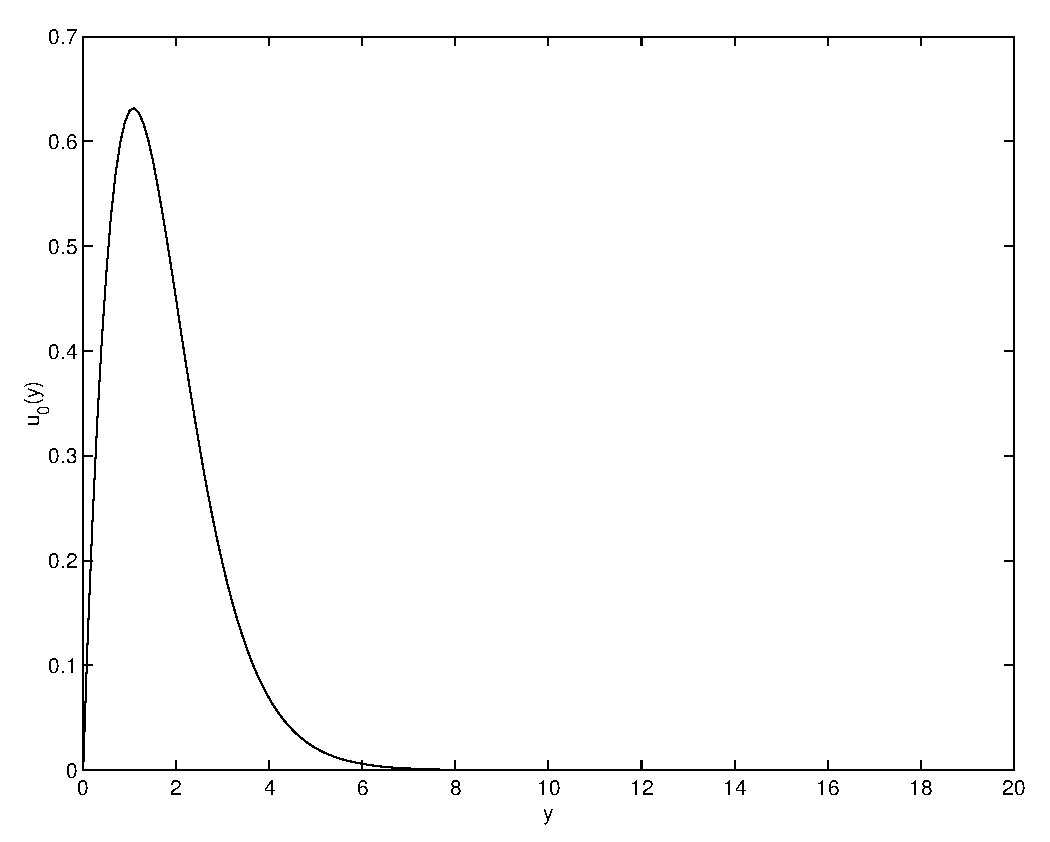
\includegraphics[width=8cm]{pics/u0prof.eps}
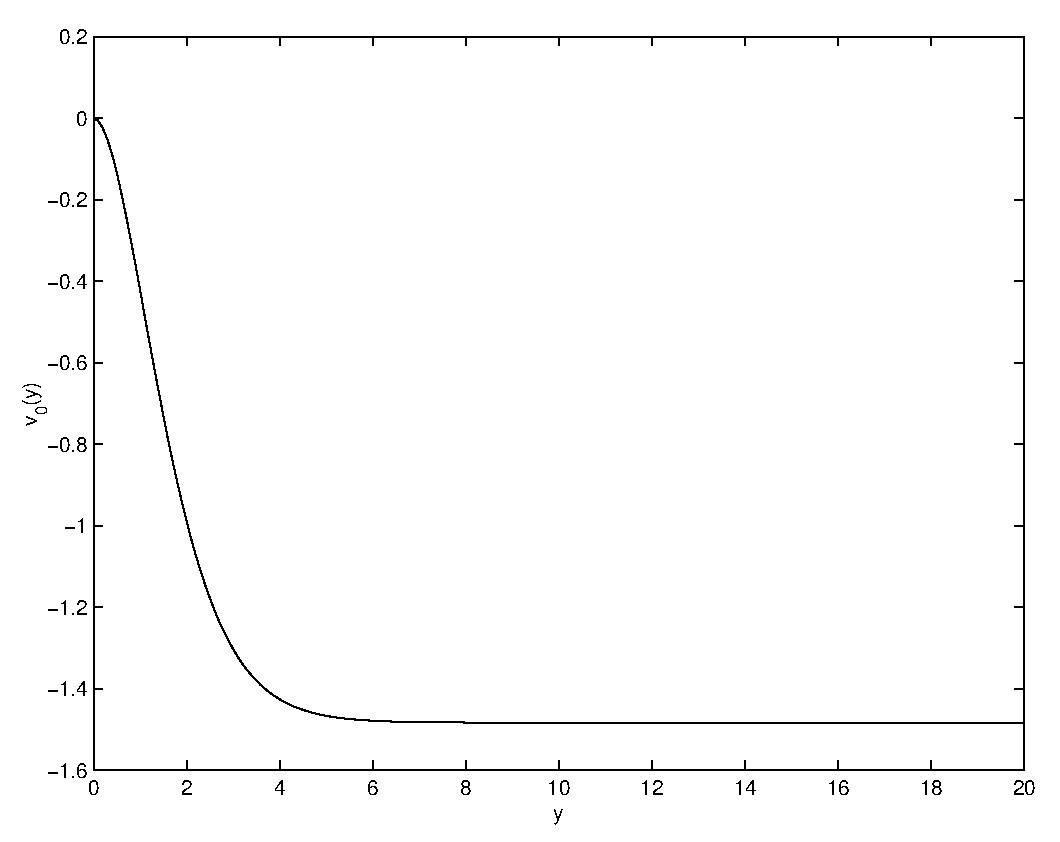
\includegraphics[width=8cm]{pics/v0prof.eps}
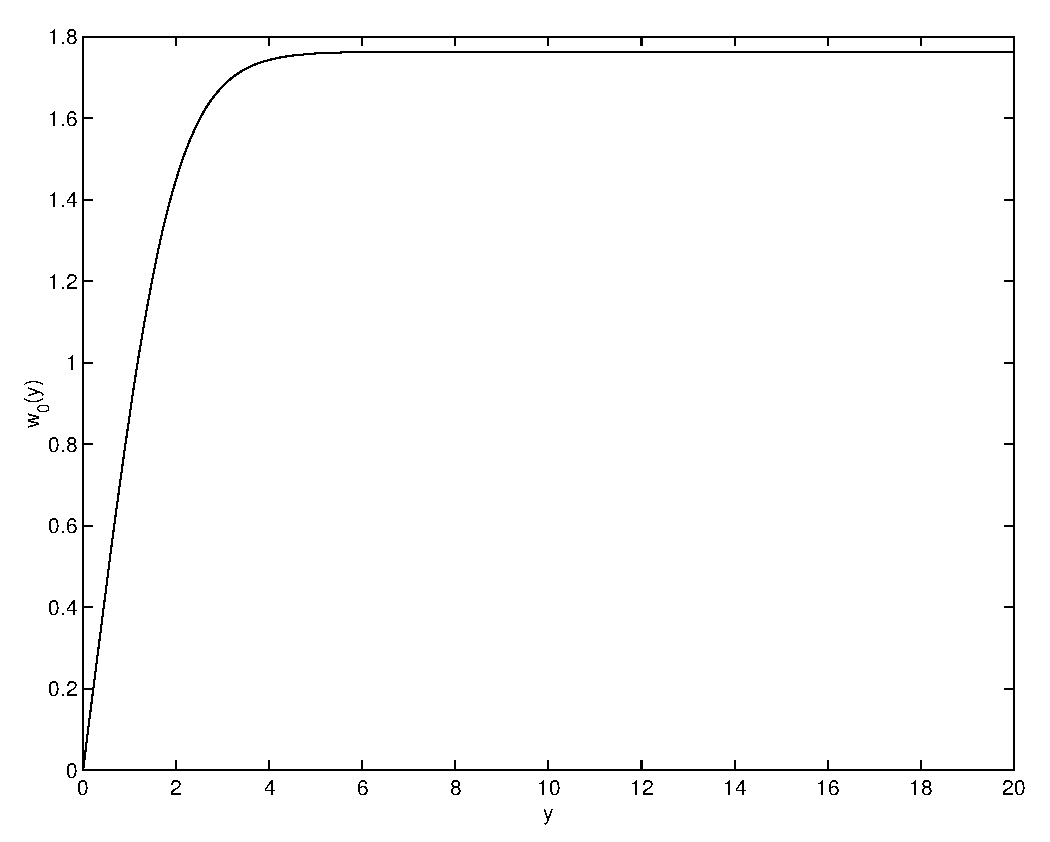
\includegraphics[width=8cm]{pics/w0prof.eps}
\caption{General profile of $k=0$ flow}
\label{zeroprofile}
\end{figure}

\begin{figure}[ht]
\centering
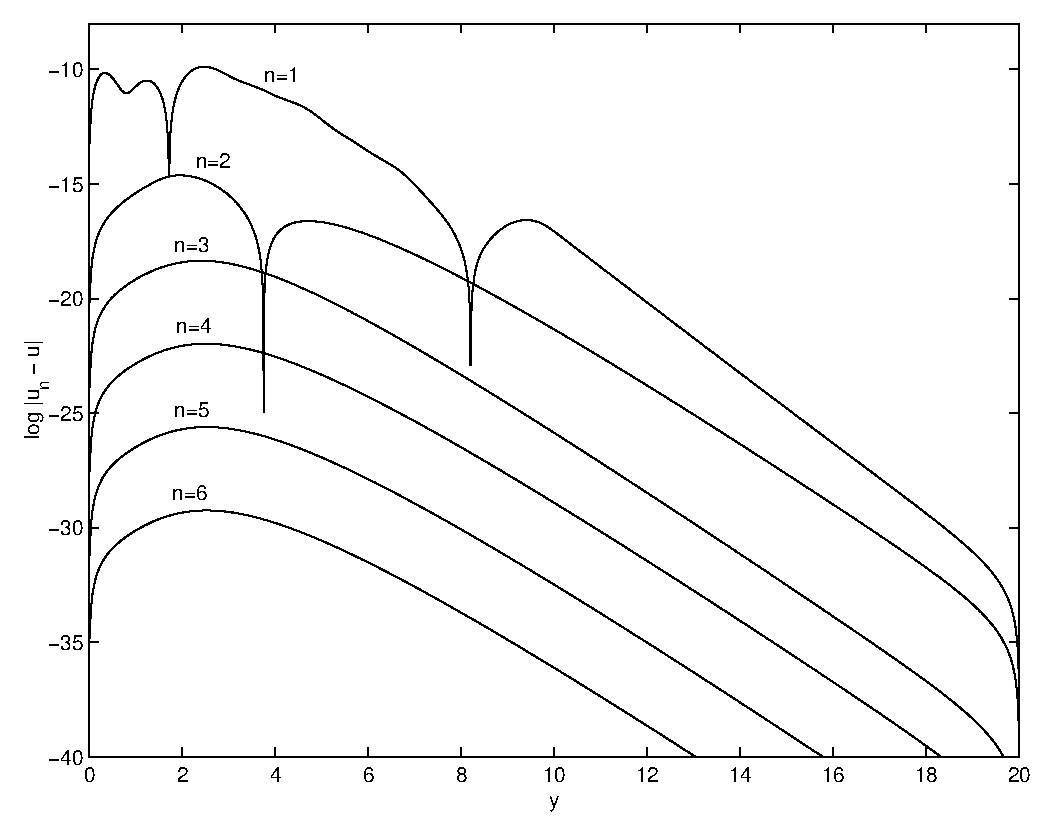
\includegraphics[width=8cm]{pics/u0iter.eps}
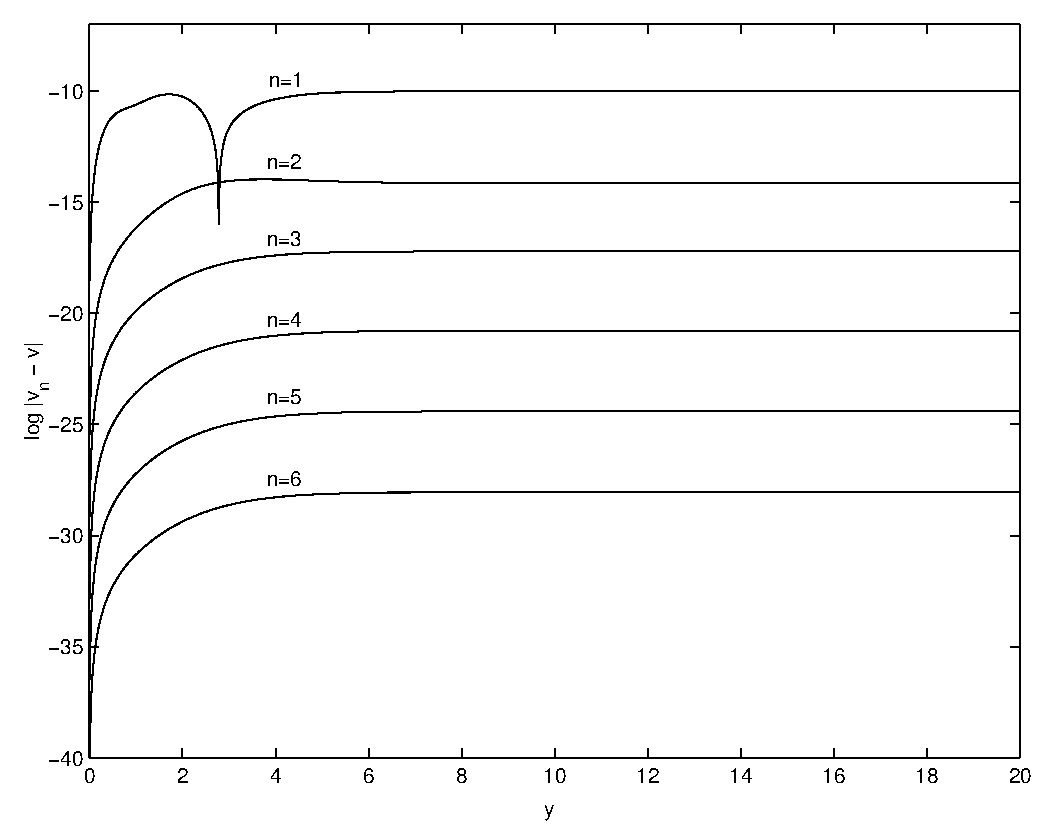
\includegraphics[width=8cm]{pics/v0iter.eps}
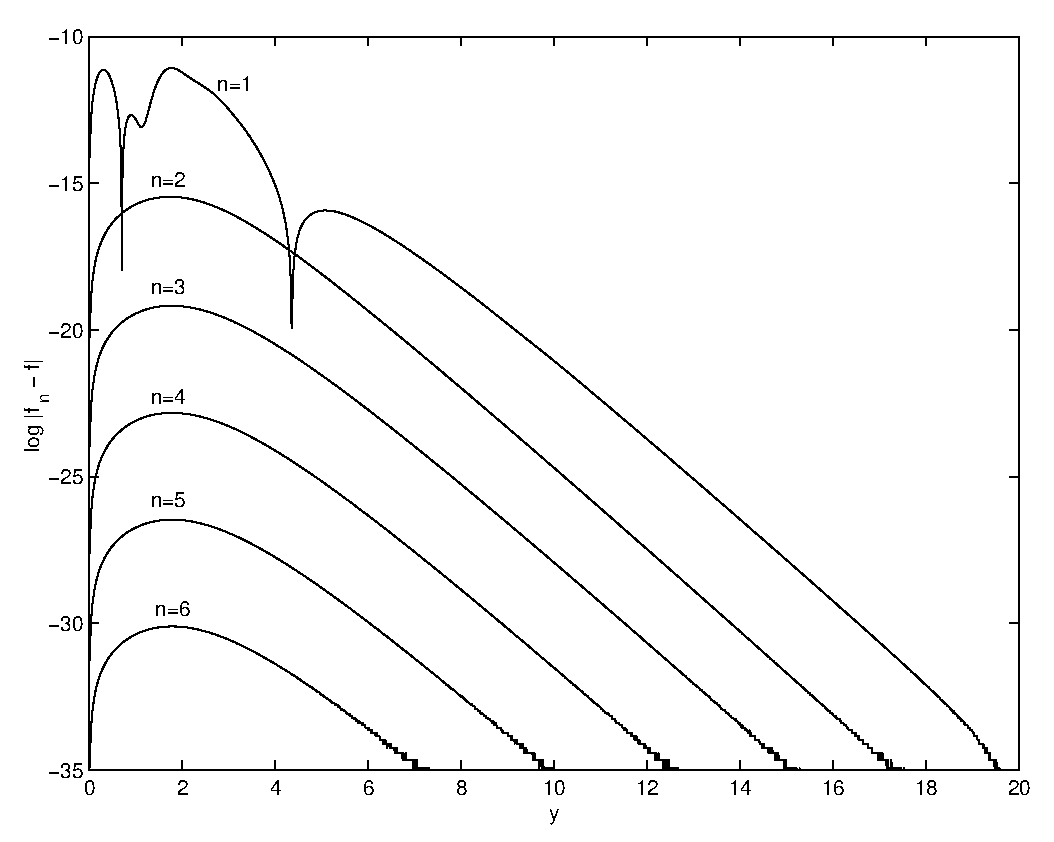
\includegraphics[width=8cm]{pics/w0iter.eps}
\caption[Error reduction for $k=0$ as number of iterations is increased]{Error reduction for the velocity components $u_0$, $v_0$, $w_0$ as the number of iterations is increased. Data obtained for $y_\infty = 20$, $h = \frac{1}{100}$. The reference state was $n=20$.}
\label{iterate}
\end{figure}

The three factors of concern are the number of iterations performed, $n$, the choice of the outer bound, $y_\infty$, and the step size, $h$. When testing the zeroth order solution, all data was calculated to quadruple precision. However, Matlab was used for the rendering, and is only capable of double precision. All data was obtained using $W_0 = 1.763$, the value proposed by Dennis and Riley.

Figures \ref{iterate} plots the logarithm of the error between a solution $f_n$ for a given number of iterations, and a reference solution which is hoped to be near the exact solution. As the figure shows, we converge on a solution after one or two iterations, and additional iterations serve to improve accuracy. The reference solution used was $n=20$, since machine precision was obtained. The block-like structures at the ends of the curves represent oscillations of the trailing digits, presumably due to roundoff error.

\begin{figure}[ht]
\centering
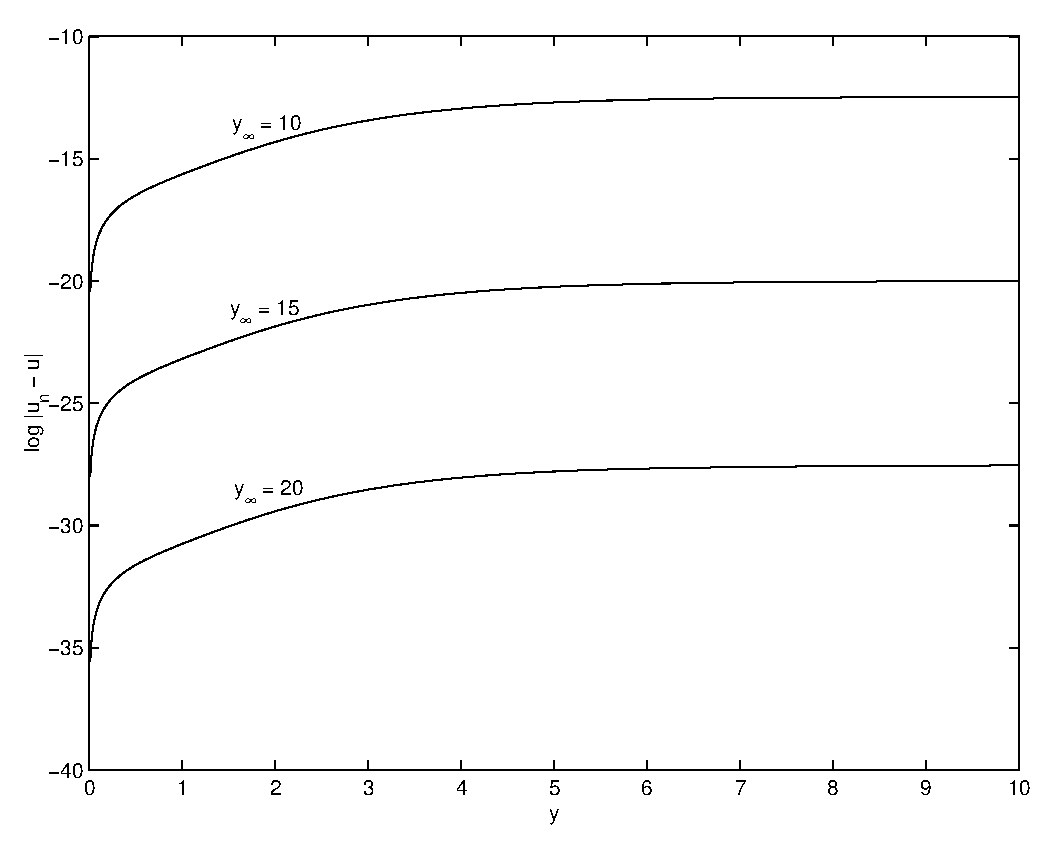
\includegraphics[width=8cm]{pics/u0inf.eps}
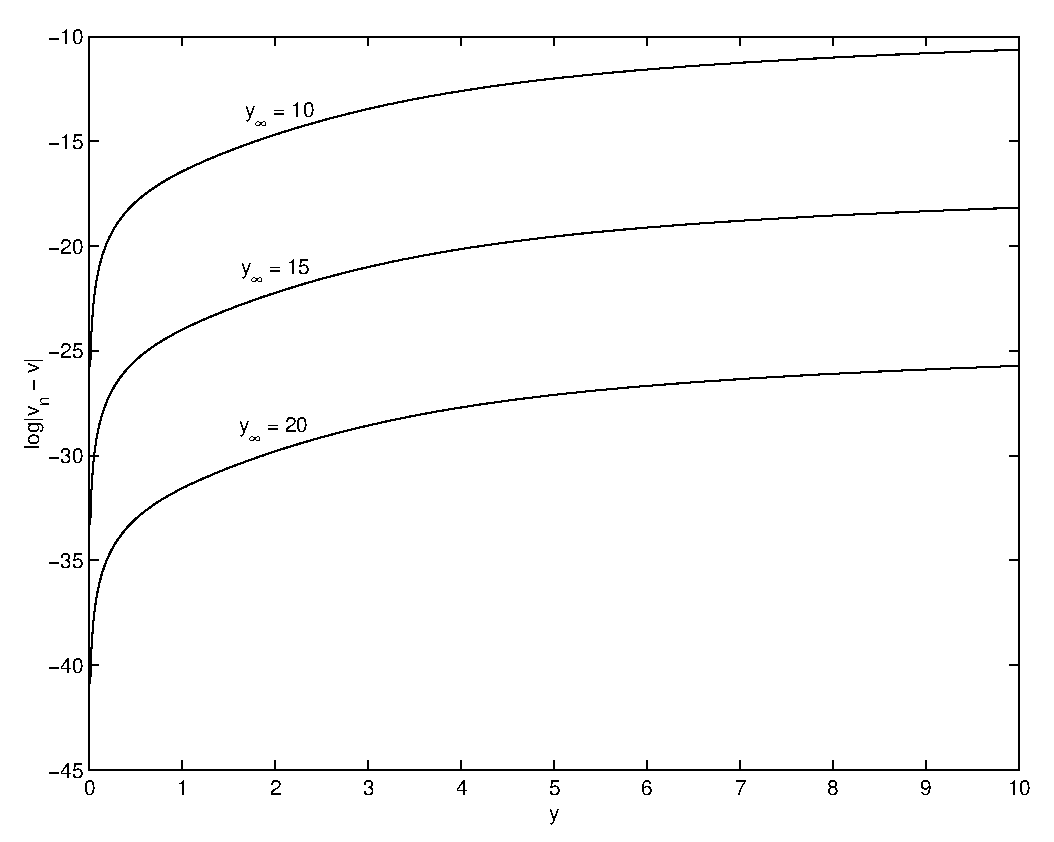
\includegraphics[width=8cm]{pics/v0inf.eps}
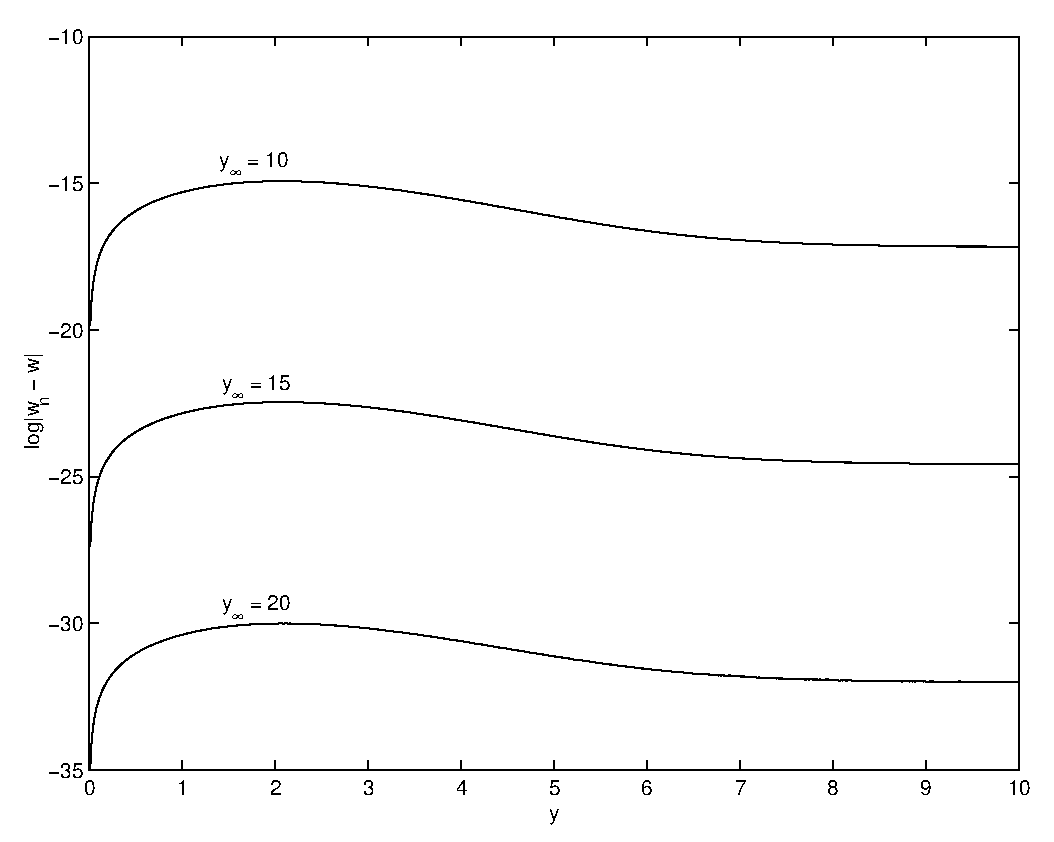
\includegraphics[width=8cm]{pics/w0inf.eps}
\caption[Error reduction for $k=0$ as $y_\infty$ is increased]{Error reduction for the velocity components $u_0$, $v_0$, $w_0$ as $y_\infty$ is increased. Data obtained for $h = \frac{1}{100}$ and $n = 8$ iterations. The reference state was $y_\infty=80$.}
\label{zeroinf}
\end{figure}

Figures \ref{zeroinf} show how the errors scale as I increase the outer bound $y_\infty$. The reference state was $y_\infty = 80$, where machine precision was obtained.

\begin{figure}[ht]
\centering
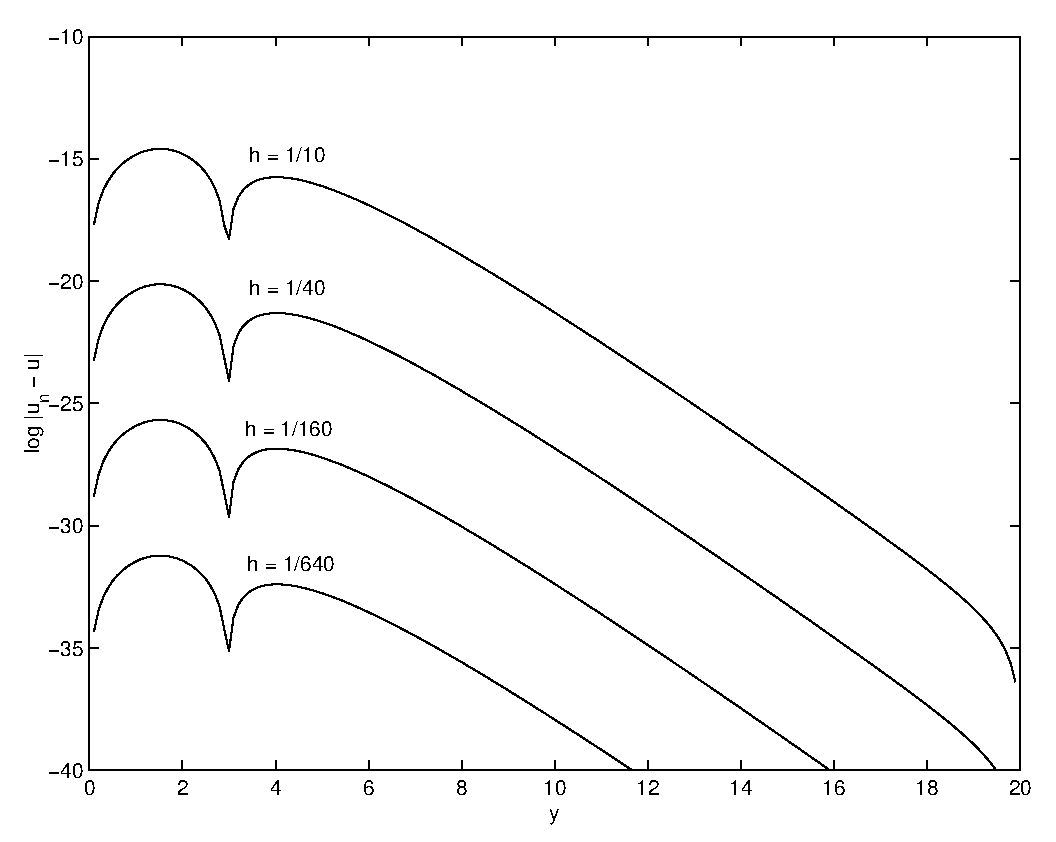
\includegraphics[width=8cm]{pics/u0h.eps}
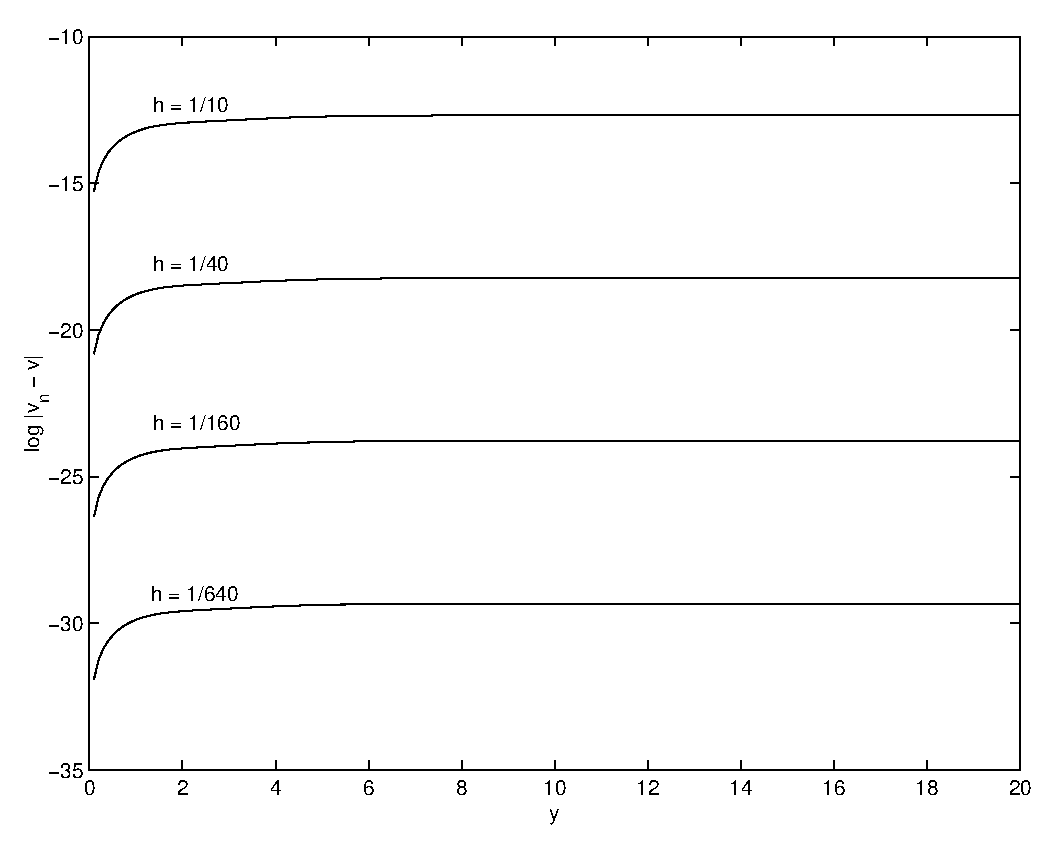
\includegraphics[width=8cm]{pics/v0h.eps}
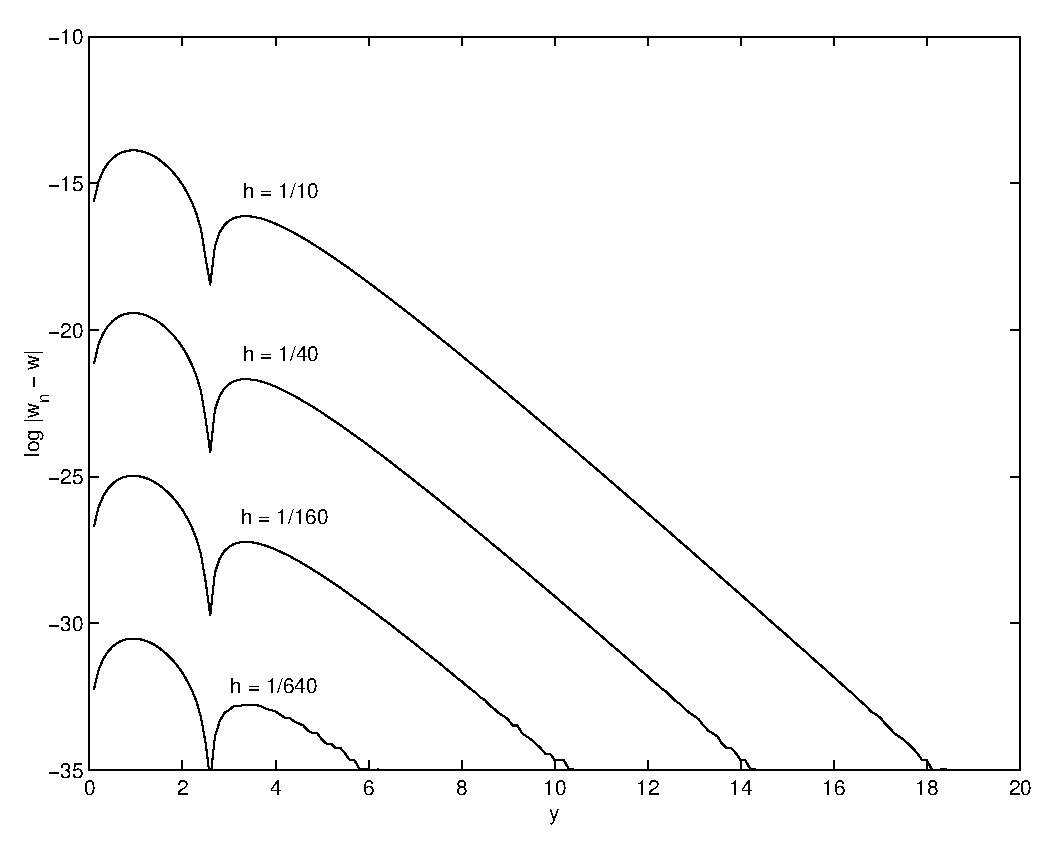
\includegraphics[width=8cm]{pics/w0h.eps}
\caption[Error reduction for $k=0$ as $h$ is decreased]{Error reduction for the velocity components $u_0$, $v_0$, $w_0$ as $h$ is decreased. Data obtained for $y_\infty = 20$ and $n = 8$ iterations. The reference state was $h = \frac{1}{3200}$.}
\label{zeroh}
\end{figure}

Figures \ref{zeroh} show how the errors scale as the step size $h$ is decreased. The reference state was $h = \frac{1}{3200}$. Although this was not the most ideal reference state, it is the most accurate solution I can obtain with a reasonable choice of $y_\infty$ and the computing resources available to me at this time.

\clearpage

\begin{figure}[t]
\centering
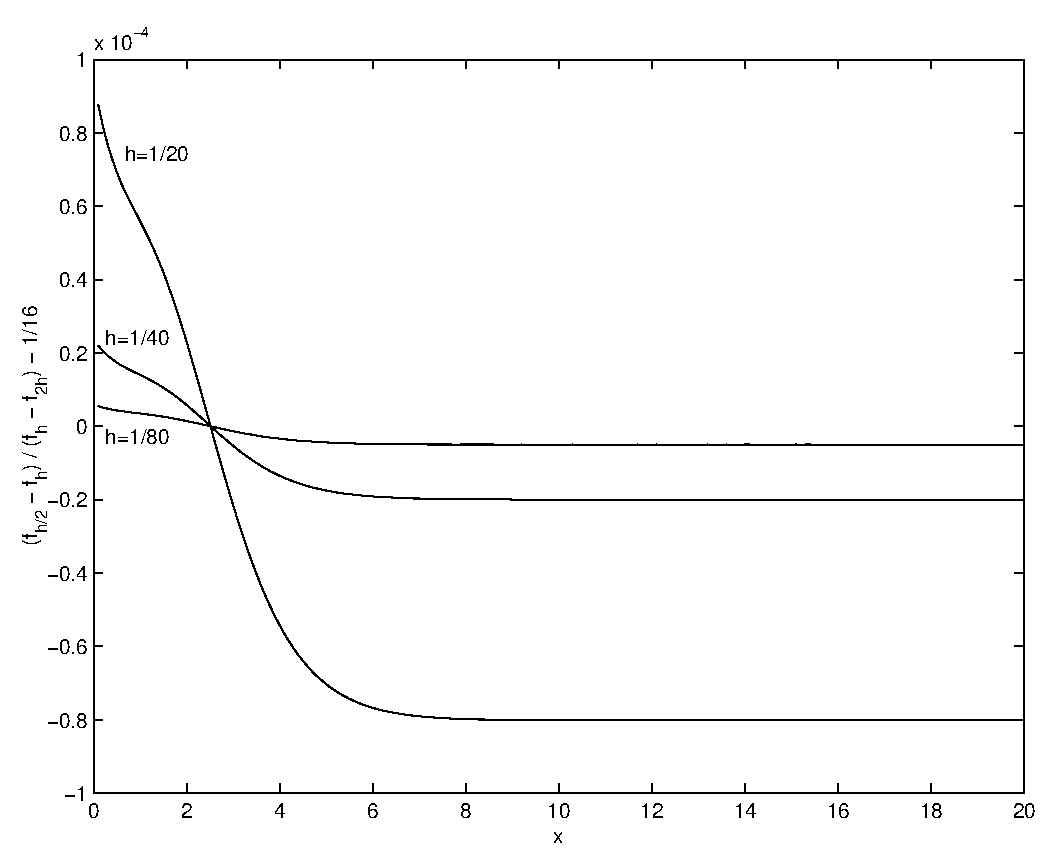
\includegraphics[width=10cm]{pics/v0ord}
\caption{Demonstration of $O(h^4)$ for $k=0$}
\label{zerohorder}
\end{figure}

Figure \ref{zerohorder} plots the function $(f_{h/2} - f_h) / (f_h - f_{2h}) - \frac{1}{16}$ where $f$ is $v_0$. If the numerical method is $O(h^4)$, then I expect that $f_h = f + Ah^4$ as $h \rightarrow 0$, where $f$ is the exact solution to the differential equation. Hence,
\begin{equation*}
\frac{f_{h/2} - f_h}{f_h - f_{2h}} = \frac{\left(\frac{1}{2}\right)^4 - 1}{1 - 2^4} = \frac{1}{16}
\end{equation*}
as $h \rightarrow 0$. Figure \ref{zerohorder} demonstrates this by showing that the ratio is both near $\frac{1}{16}$, by the small amplitude, and that the variation from this value is reduced as $h$ decreases.

The most difficult problem in solving the zeroth order equations involved the initial guess for the desirable solution. Being nonlinear, it is possible that there are nonunique solutions to the equations. Based on the equation $v_0' = -u_0$, it was required that $u_0$ be positive for the majority of the range of $y$, if not the entire range. But if the initial guess was poor, then the iterative solution had a tendency to find solutions where $u_0 < 0$ for large values of $y$, causing $v_0$ to exponentially increase.

This problem was remedied through the use of cubic spline interpolation curves between a series of 11 nodes from $y = 0$ to $y = 10$. For $W_0 = 1.763$, these nodes were calculated for the case of $y_\infty = 10$. But for other values of $W_0$, these nodes only provided a stable solution for about $W_0 = 1.763 \pm 1$. For lower values of $W_0$, I calculated the respective nodes for $W_0 = 1$, which provided a similar solution where the profiles have the same structure and $u_0 > 0$ everywhere. Although I lack a clear algorithm, this process can be extended to obtain solutions for an arbitrary value of $W_0$.

\section{Numerical results for $k>0$}

Numerical data collected for $k>0$ is currently not as reliable as the previous case. Doubts about the validity of the higher order solutions have arisen since the following data was calculated. However, a future analysis will most likely follow a similar procedure and may produce analogous results. Also, since the method was only $O(h^2)$ accurate, data was only calculated to double precision.

The chief difficulty in calculating the higher order solutions seems to be due to the need for accuracy in the trailing digits. Because the fluctuations in the higher order solutions can extend for moderately large values of $y$, a similarly large choice for $y_\infty$ is needed for convergence. However, since larger values of $y_\infty$ tend to achieve machine precision at exponential tails of the solutions, vital trailing digits (necessary when the behavior depends on very small fluctuations) are lost in roundoff error, which eventually leads to abnormally large results. Typically, the solutions in their native form cannot be solved beyond about $k=5$ with double precision. The situation is only moderately improved in quadruple precision, to about $k=10$. Although an $O(h^4)$ method would most likely improve this situation, it's not a reliable solution. An alternative which may be more successful is the improvement of the $u_k=0$ boundary condition at $y_\infty$, which could possibly be re-expressed in terms of an asymptotic solution to the differential equations.

The modification used here was a rescaling of the quantities by an amount $\lambda$ so that
\begin{equation*}
u = \sum_{k=0}^\infty u_k x^{2k+1} = \sum_{k=0}^\infty u_k \lambda^{2k+1} \left(\frac{x}{\lambda}\right)^{2k+1} = \sum_{k=0}^\infty \tilde{u}_k \tilde{x}^{2k+1}
\end{equation*}
where $\tilde{u}_k = u_k \lambda^{2k+1}$ and $\tilde{x}^{2k+1} = \left(x/\lambda\right)^{2k+1}$. Similar transformations apply to $v$, $w$, and $W$, except the $2k+1$'s become $2k$'s. The hope is that this rescaling will increase the quantities and that critical trailing digits are not lost.

The quantity of interest here is $W$ evaluated at $x=\pi$. A more thorough analysis should be performed over a range of values of $x$. Additionally, the velocity profiles within the boundary layer should also be examined. But this is a succinct test with some merit.

Figures \ref{wcvary} and \ref{wcvarybad} shows how $W(\pi)$ varies as $W_0$ is changed. Figure \ref{wcvary} shows the general linear behavior of $W(\pi)$. The most notable feature is that $W(\pi) \neq 0$ when $W_0 = 1.763$. Using a crude linear regression curve, an approximate value for $W_0$ is found to be $1.063$.

Figure \ref{wcvarybad} includes points which were omitted from figure \ref{wcvary} because of their unusual behavior. A number of values near $W_0 = 1.3$ were calculated, and $W(\pi)$ was shown to rapidly vary in this region. A positively divergent value was found for $W_0 = 1.325$, but many negative values for $W(\pi)$ were also calculated. No order was found in the variation, which can only be assumed to be rapidly oscillatory, if exhibiting any pattern at all. A very large number of points would be necessary to produce a smooth profile. This region could be due to some interesting behavior of the system, but is more likely a consequence of either a breakdown of the numerical method, or simply an error in the calculation. Further study should be conducted to determine the origin of this behavior.

\clearpage

\begin{figure}[tp]
\centering
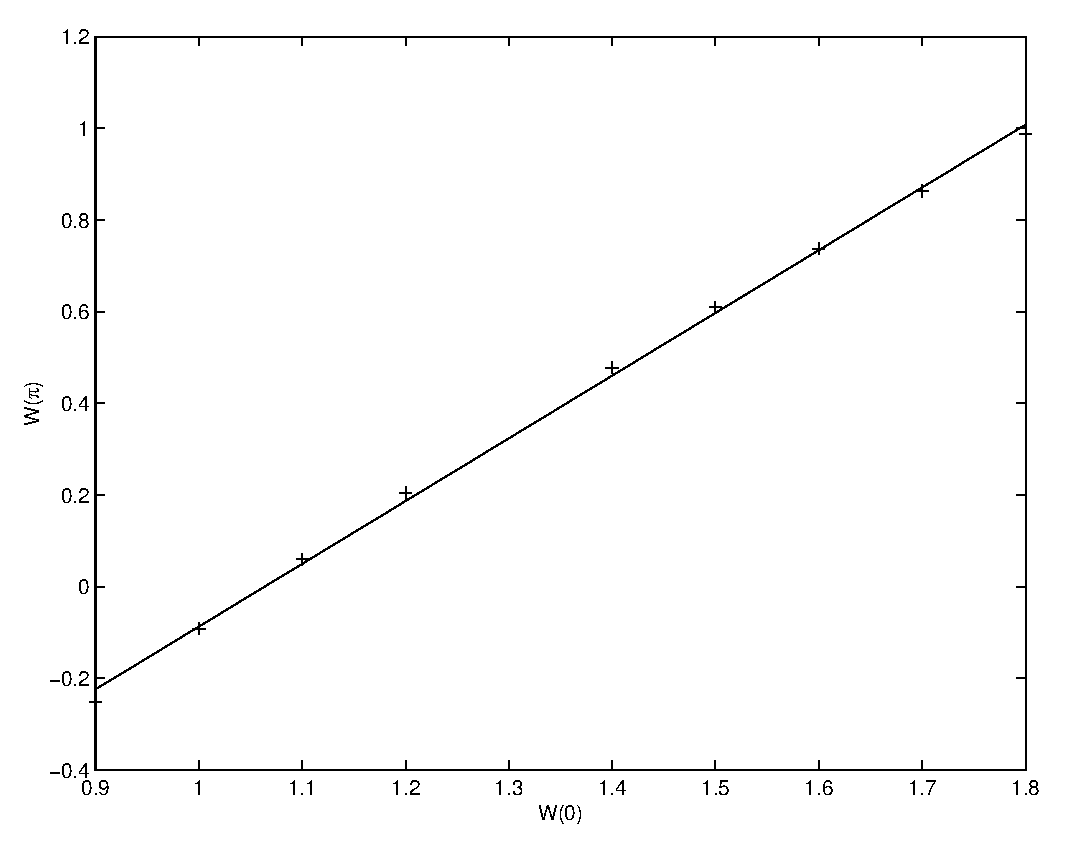
\includegraphics[width=10cm]{pics/wcpi.eps}
\caption[Plot of $W(\pi)$ versus $W_0$]{Variation of $W(\pi)$ as $W_0$ is changed, with a linear regression curve across the stable points. Numbers calculated for $y_\infty = 40$, $h = \frac{1}{100}$, $\lambda = 10^{-5}$, $k=20$.}
\label{wcvary}
\end{figure}

\begin{figure}[p]
\centering
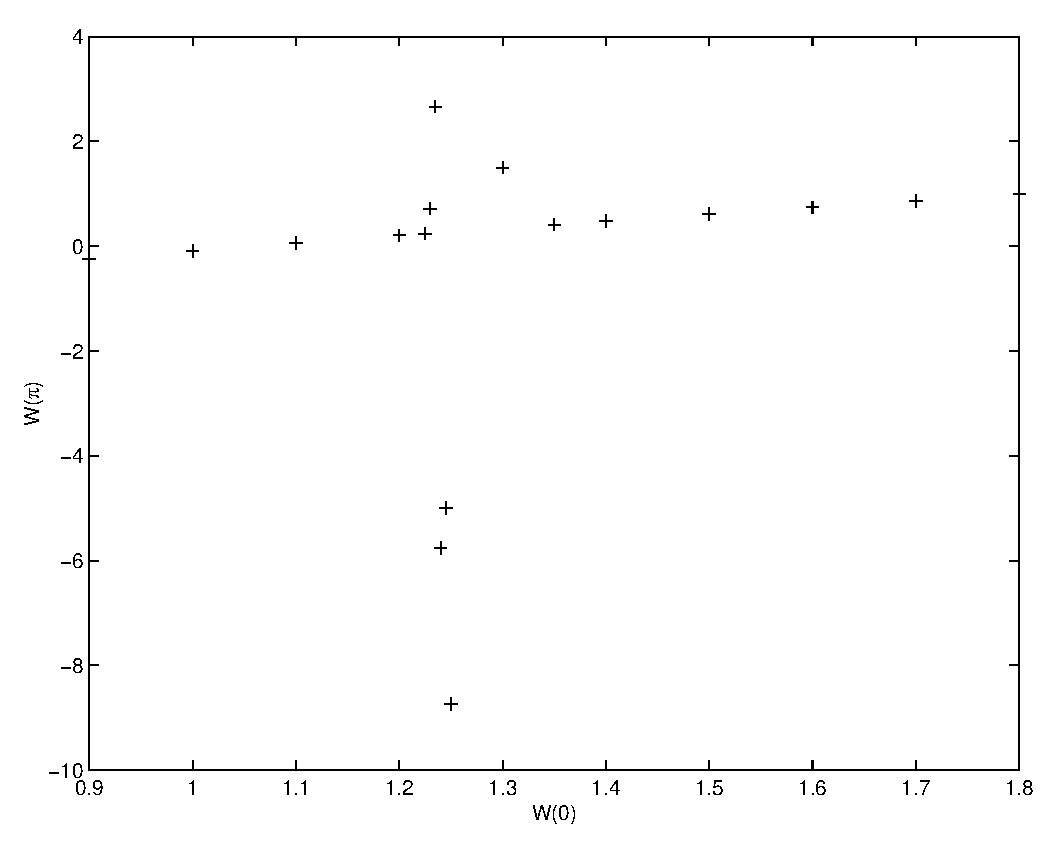
\includegraphics[width=10cm]{pics/wcpi_bad.eps}
\caption[Plot of $W(\pi)$ versus $W_0$, including unstable region]{Figure \ref{wcvary}, with the inclusion of points within the unstable region near $W_0 = 1.3$.}
\label{wcvarybad}
\end{figure}

\clearpage

This next set of data shows that the value of $W$ calculated at $x=\pi$ has errors which scale appropriately for some particular value of $W_0$, namely $W_0 = 1.5$. The intention was to choose a value which was both far from the zero value $W_0 = 1.063$, the unstable region $W_0 = 1.3$, and the proposed result by Dennis and Riley, $W_0 = 1.763$. The dependencies to be examined are the outer bound $y_\infty$, the step size $h$, the scaling parameter $\lambda$, and the order $k$.

\begin{figure}[h]
\centering
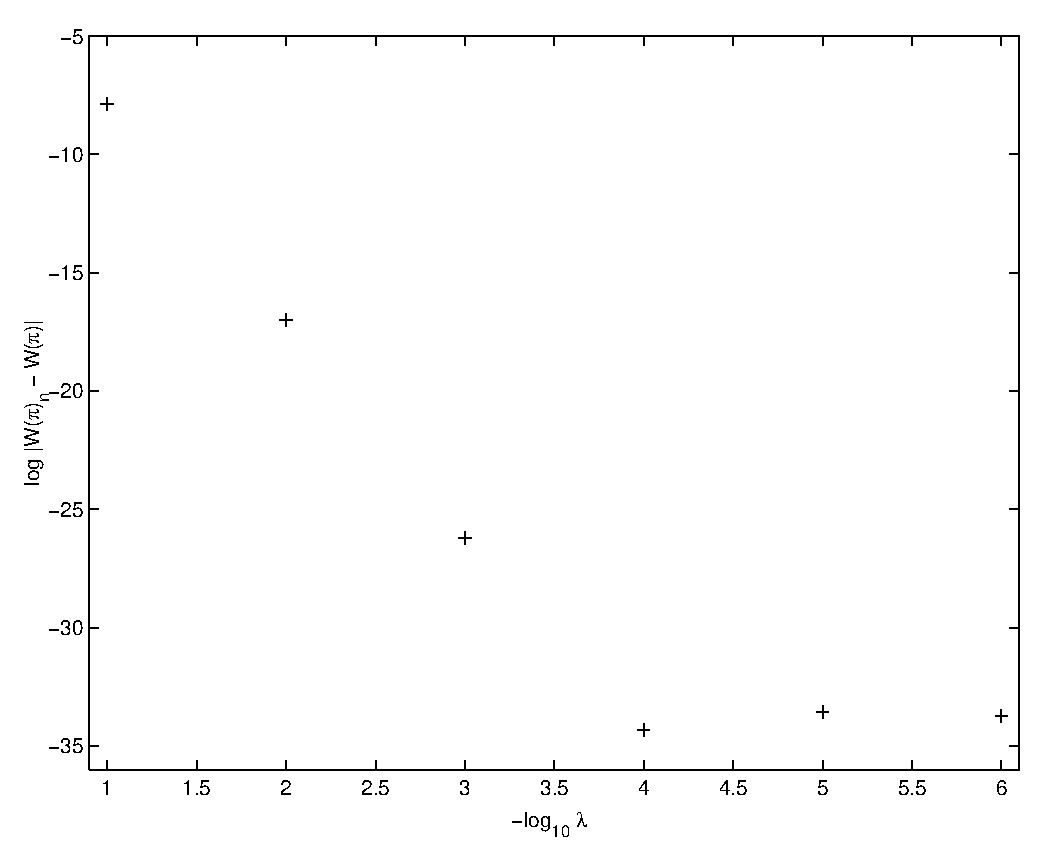
\includegraphics[width=10cm]{pics/wcpi_scale.eps}
\caption[Independence of scale for $W(\pi)$]{Independence of scale for $W(\pi)$ as $\lambda$ is decreased. Numbers calculated for $y_\infty=40$, $h = \frac{1}{100}$, $k=20$.}
\label{wcscale}
\end{figure}

Figure \ref{wcscale} shows how $W(\pi)$ converges to a result which is independent of scale as $\lambda$ is reduced by factors of 10. Errors are calculated with reference to the $\lambda = 10^{-7}$ solution. Although the result purports to establish this independence of scale, I am concerned that this extreme reduction of $\lambda$ is simply reducing terms in the differential equations to negligible values, and consequently obtaining leading order results which may not in fact be accurate. Unfortunately, I lacked sufficient time to explore this possibility.

An important observation of this plot is that the errors don't go below about $10^{-15}$ (or $\textrm{e}^{-35}$). This is almost definitely due to either the limit of double precision arithmetic in the calculation or in Matlab. Calculations performed in quadruple precision can be pushed beyond this for greater accuracy.

\begin{figure}[p]
\centering
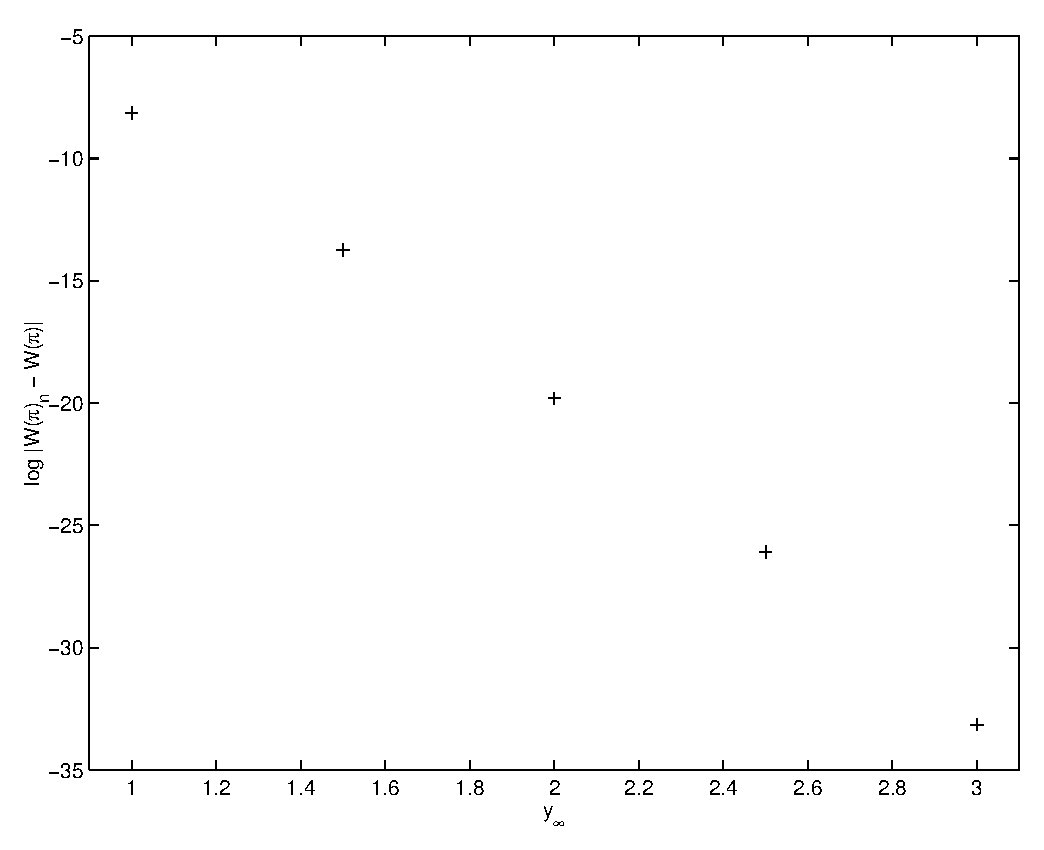
\includegraphics[width=10cm]{pics/wcpi_inf.eps}
\caption[Reduction of errors in $W(\pi)$ with increase of $y_\infty$]{Reduction of errors in $W(\pi)$ as $y_\infty$ is increased. Numbers calculated for $h = \frac{1}{100}$, $\lambda = 10^{-5}$, $k=20$.}
\label{wcinfty}
\end{figure}


Figure \ref{wcinfty} demonstrates that errors in $W(\pi)$ are exponentially reduced as $y_\infty$ approaches infinity. The reference solution uses $y_\infty = 80$, where machine precision is obtained.

\begin{figure}[p]
\centering
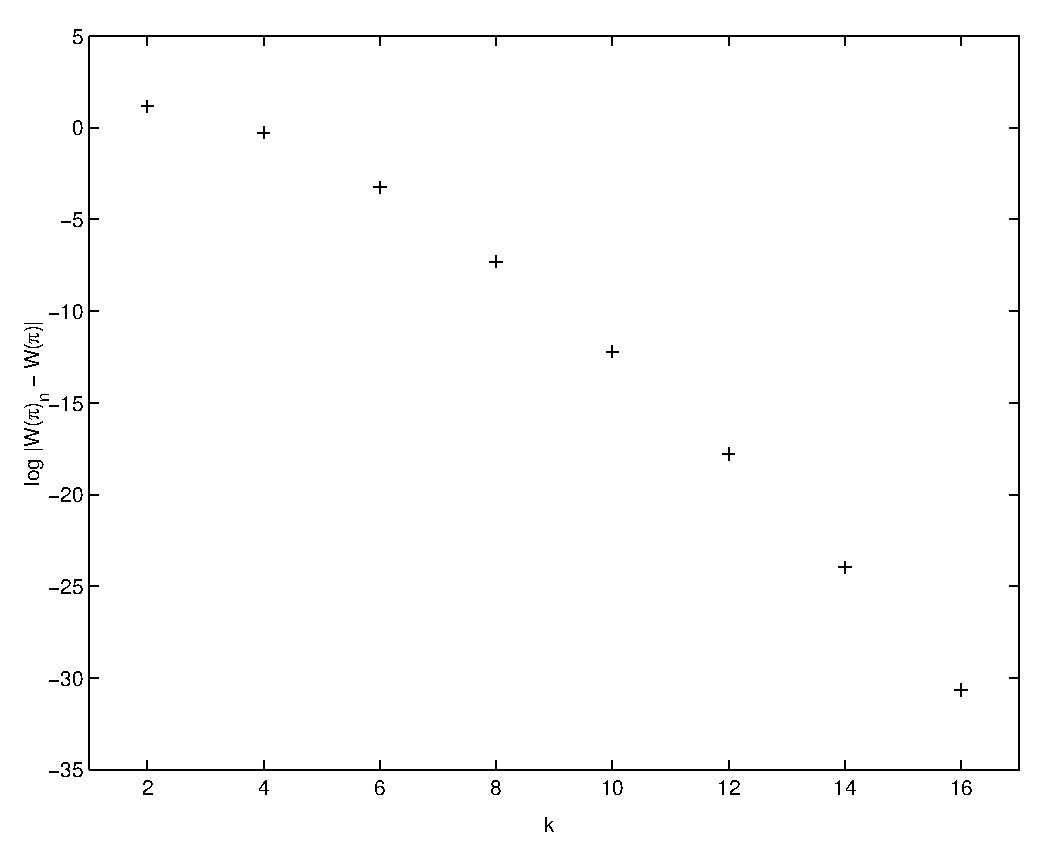
\includegraphics[width=10cm]{pics/wcpi_ord.eps}
\caption[Reduction of errors in $W(\pi)$ when calculated to higher orders]{Reduction of errors in $W(\pi)$ when calculated to higher orders. Numbers calculated for $y_\infty=40$, $h = \frac{1}{100}$, $\lambda = 10^{-5}$.}
\label{wcorder}
\end{figure}

Figure \ref{wcorder} yields a similar result, with $W(\pi)$'s errors reducing exponentially as it is calculated to higher order. The reference solution is to $k=25$ order, which achieves machine precision.

\clearpage

\begin{figure}[ht]
\centering
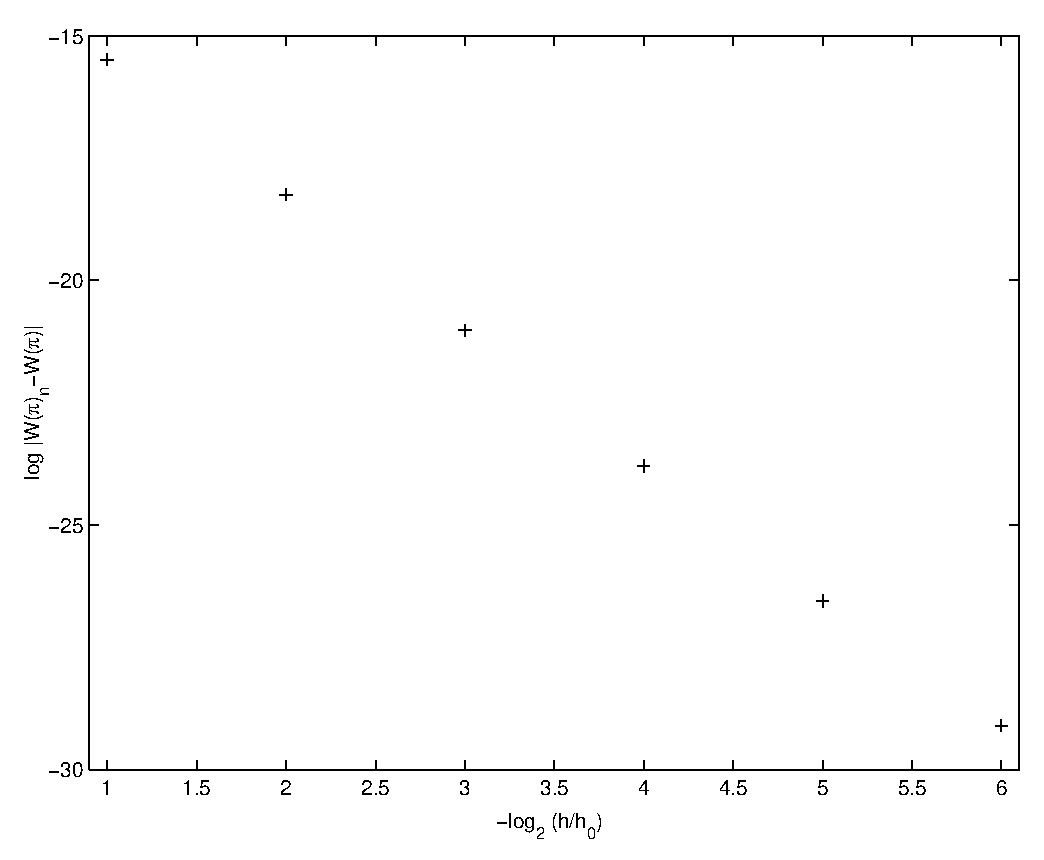
\includegraphics[width=10cm]{pics/wcpi_h.eps}
\caption[Reduction of errors in $W(\pi)$ with decrease of $h$]{Reduction of errors in $W(\pi)$ at smaller step size $h$. Numbers calculated for $y_\infty=20$, $\lambda = 10^{-5}$, $k=20$.}
\label{wcstep}
\end{figure}

Finally, Figure \ref{wcstep} shows that $W(\pi)$ has exponentially decreasing errors as the step size $h$ is decreased in powers of 2, from $h=\frac{1}{10}$ to $h=\frac{1}{320}$. Like with $k=0$, the reference state used was $h = \frac{1}{3200}$, with $y_\infty$ being reduced from $40$ to $20$ in order to study a wider range of values. In fact, since the method is order $O(h^2)$, the potential difficulties of studying variations in $h$ are even greater here than in the case of $k=0$. Also, the errors were not explicitly shown to be $O(h^2)$ accurate, but can in principle be inferred from this plot.

As mentioned before, I have marginal confidence in these results. I have been unable to obtain convincing evidence supporting the validity of the solutions for the velocity components at higher orders. Since $W$ depends directly on $u$ and indirectly on all three components, it casts doubt on any values calculated for $W(\pi)$. Although the result that $W_0 \neq 1.763$ is interesting, I believe that the velocity components must be clearly identified before any values of $W(\pi)$ can be taken seriously.

Nonetheless, this analysis can be performed on any solution once the higher order velocities have been determined with confidence, and can be used to determine $W(\pi)$, as well as the more revealing possibility of $u =0$ for all $y$ when $x = \pi$.

\chapter{Conclusion}
I've provided a clear derivation of the boundary layer model which was presented by Dennis and Riley. Using this model, I performed a series extension whereby I reduced the resulting partial differential equations to a series of ordinary differential equations. By solving the equation at each order, I should in principle be able to construct a solution which can be extended from the outer end of the pipe to the inner end, where accuracy towards the inner end is improved by solving for higher order terms in the series. As a result of this analysis, I should have a complete solution for the flow across the entire boundary layer.

Although I was able to produce a satisfactory solution to the zeroth order nonlinear equations and hence determine the flow at the outer end of the pipe, I lacked the experience or talent to overcome the numerical difficulties presented by the higher order equations, and could not obtain confident solutions beyond more than a few orders in the series expansion. But I have presented a clear analysis which can be performed to analyze the results and check their validity.

Using the results from the zeroth order equations, I can currently calculate certain constants of interest, such as the asymptotic value of $v_0$ as $y \rightarrow \infty$, to a very high level of accuracy. Such constants may be of importance in asymptotic solutions for the flow in this region.

If, in the future, I am able to solve the higher order equations with confidence, then I can study the structure of the flow across the pipe as a whole. In particular, I can study the entrainment of fluid across the boundary layer, and can determine whether the boundary layer is depleted as I move toward the outer end. I would also be able to determine whether any stagnation points exist in the boundary layer.

Additionally, I can construct a $O(h^4)$ accurate solution for the higher orders, as done for the zeroth order equations. With a complete solution of the boundary layer flow at this level of precision, it will be possible to provide numerical evidence which can determine the accuracy of proposed asymptotic solutions for the flow across the entire pipe.

In conclusion, although I did not obtain a satisfactory solution, the scattered successes here provide hope that this method can be corrected or modified to produce a precise numerical solution to the boundary layer equations. This numerical solution can then be used to determine the validity of any proposed asymptotic solutions for the system.

\begin{thebibliography}{99}

\bibitem{dea27}Dean, W. R. (1927), Note on the motion of fluid in a curved pipe. \textit{Phil. Mag.} \textbf{4}, 208--223.

\bibitem{dea28}Dean, W. R. (1927), The streamline motion of fluid in a curved pipe. \textit{Phil. Mag.} \textbf{5}, 673--695.

\bibitem{den80}Dennis, S. C. R. (1980), Calculation of the steady flow through a curved tube using a new finite-difference method. \textit{J. Fluid Mech.} \textbf{99}, 449--467.

\bibitem{den82}Dennis, S. C. R. \& Ng, M. (1982), Dual solutions for steady laminar flow through a curved tube. \textit{Q. Jl. Mech. appl. Math.} \textbf{35}, 305--324.

\bibitem{ito69}Ito, H. (1969), Laminar flow in curved pipes. \textit{Z. angew Math. Mech.} \textbf{49}, 653--663.

\bibitem{smi76}Smith, F. T. (1976), Steady motion within a curved pipe. \textrm{Proc. R. Soc. Lond.} A \textbf{347}, 345--370.

\bibitem{jay91} Jayanti S. \& Hewitt J. F. (1991), On the paradox concerning friction factor ratio in laminar flow in coils, \textit{Proc. R. Soc. Lond.} A \textbf{432}, 291--299.

\bibitem{den91}Dennis, S. C. R. \& Riley N. (1991), On the fully developed flow in a curved pipe at large Dean number, \textit{Proc. R. Soc. Lond.} A \textbf{434}, 473--478.

\bibitem{isr96}Iserles, A. (1996), \textit{A First Course in the Numerical Analysis of Differential Equations}, Cambridge University Press, Cambridge.

\bibitem{num1}Burden, R. L. \& Faires, J. D. (1993), \textit{Numerical Analysis}, PWS-KENT, Boston, MA.

\bibitem{num2}Gerald, C. F. \& Wheatley, P. O. (1989), \textit{Applied Numerical Analysis}, Addison-Wesley, Reading, MA.

\end{thebibliography}

\end{document}